\documentclass{article}
\usepackage{graphicx}
\usepackage{amsmath}
\graphicspath{ {images/} }
\usepackage{amssymb}
\usepackage[left=3cm,top=2cm,right=3cm,nohead,nofoot]{geometry}
\usepackage{latexsym}
\usepackage{epsfig}
\parindent0pt
\parskip6pt
\usepackage[section]{placeins}
\pagestyle{empty}
\usepackage{pstcol}
\newcommand{\R}{{\mathbb R}}

\title{MATH 444 Problem Set 1}
\author{Connor Wolfe}
\begin{document}
\maketitle

\pagebreak
\section*{Problem 1}

\subsection*{Overview}
The first problem asks us to analyze the file 'ModelReductionData.mat.' This file contains maxtrix X (6x4000) which contains 4,000 samples of 6-dimensional data.    The first part of the problem will focus on graphing of high dimensional data.  The second part of the problem will begin to explore mathematical concepts of SVD, singular value, and principal components.

\subsection*{Part (a)}
We are asked to use scatter plots to visualize each dimension of the data versus every other dimension.  Since there are 6 dimensions, there are 15 permutations of dimension pairs we need to plot.  In order to plot every dimension I made a nested for loop to iterate 'i' from 1:5 and 'j' from 'i':6. It is trivial to see this will produce 15 pairings of i and j.  Once inside the for loops with indices for both dimensions, I plotted following the template on the assignment sheet.  The operative line of code is to plot dimension i vs j is :
\begin{verbatim}7: plot(X(i,:),X(j,:), 'k.', 'MarkerSize',7);\end{verbatim}
The rest of the lines in the for loop are for formatting purposes only.  The resulting 15 plots are shown in figure (1).  

 \begin{figure}[h!]
    \centerline
    {
    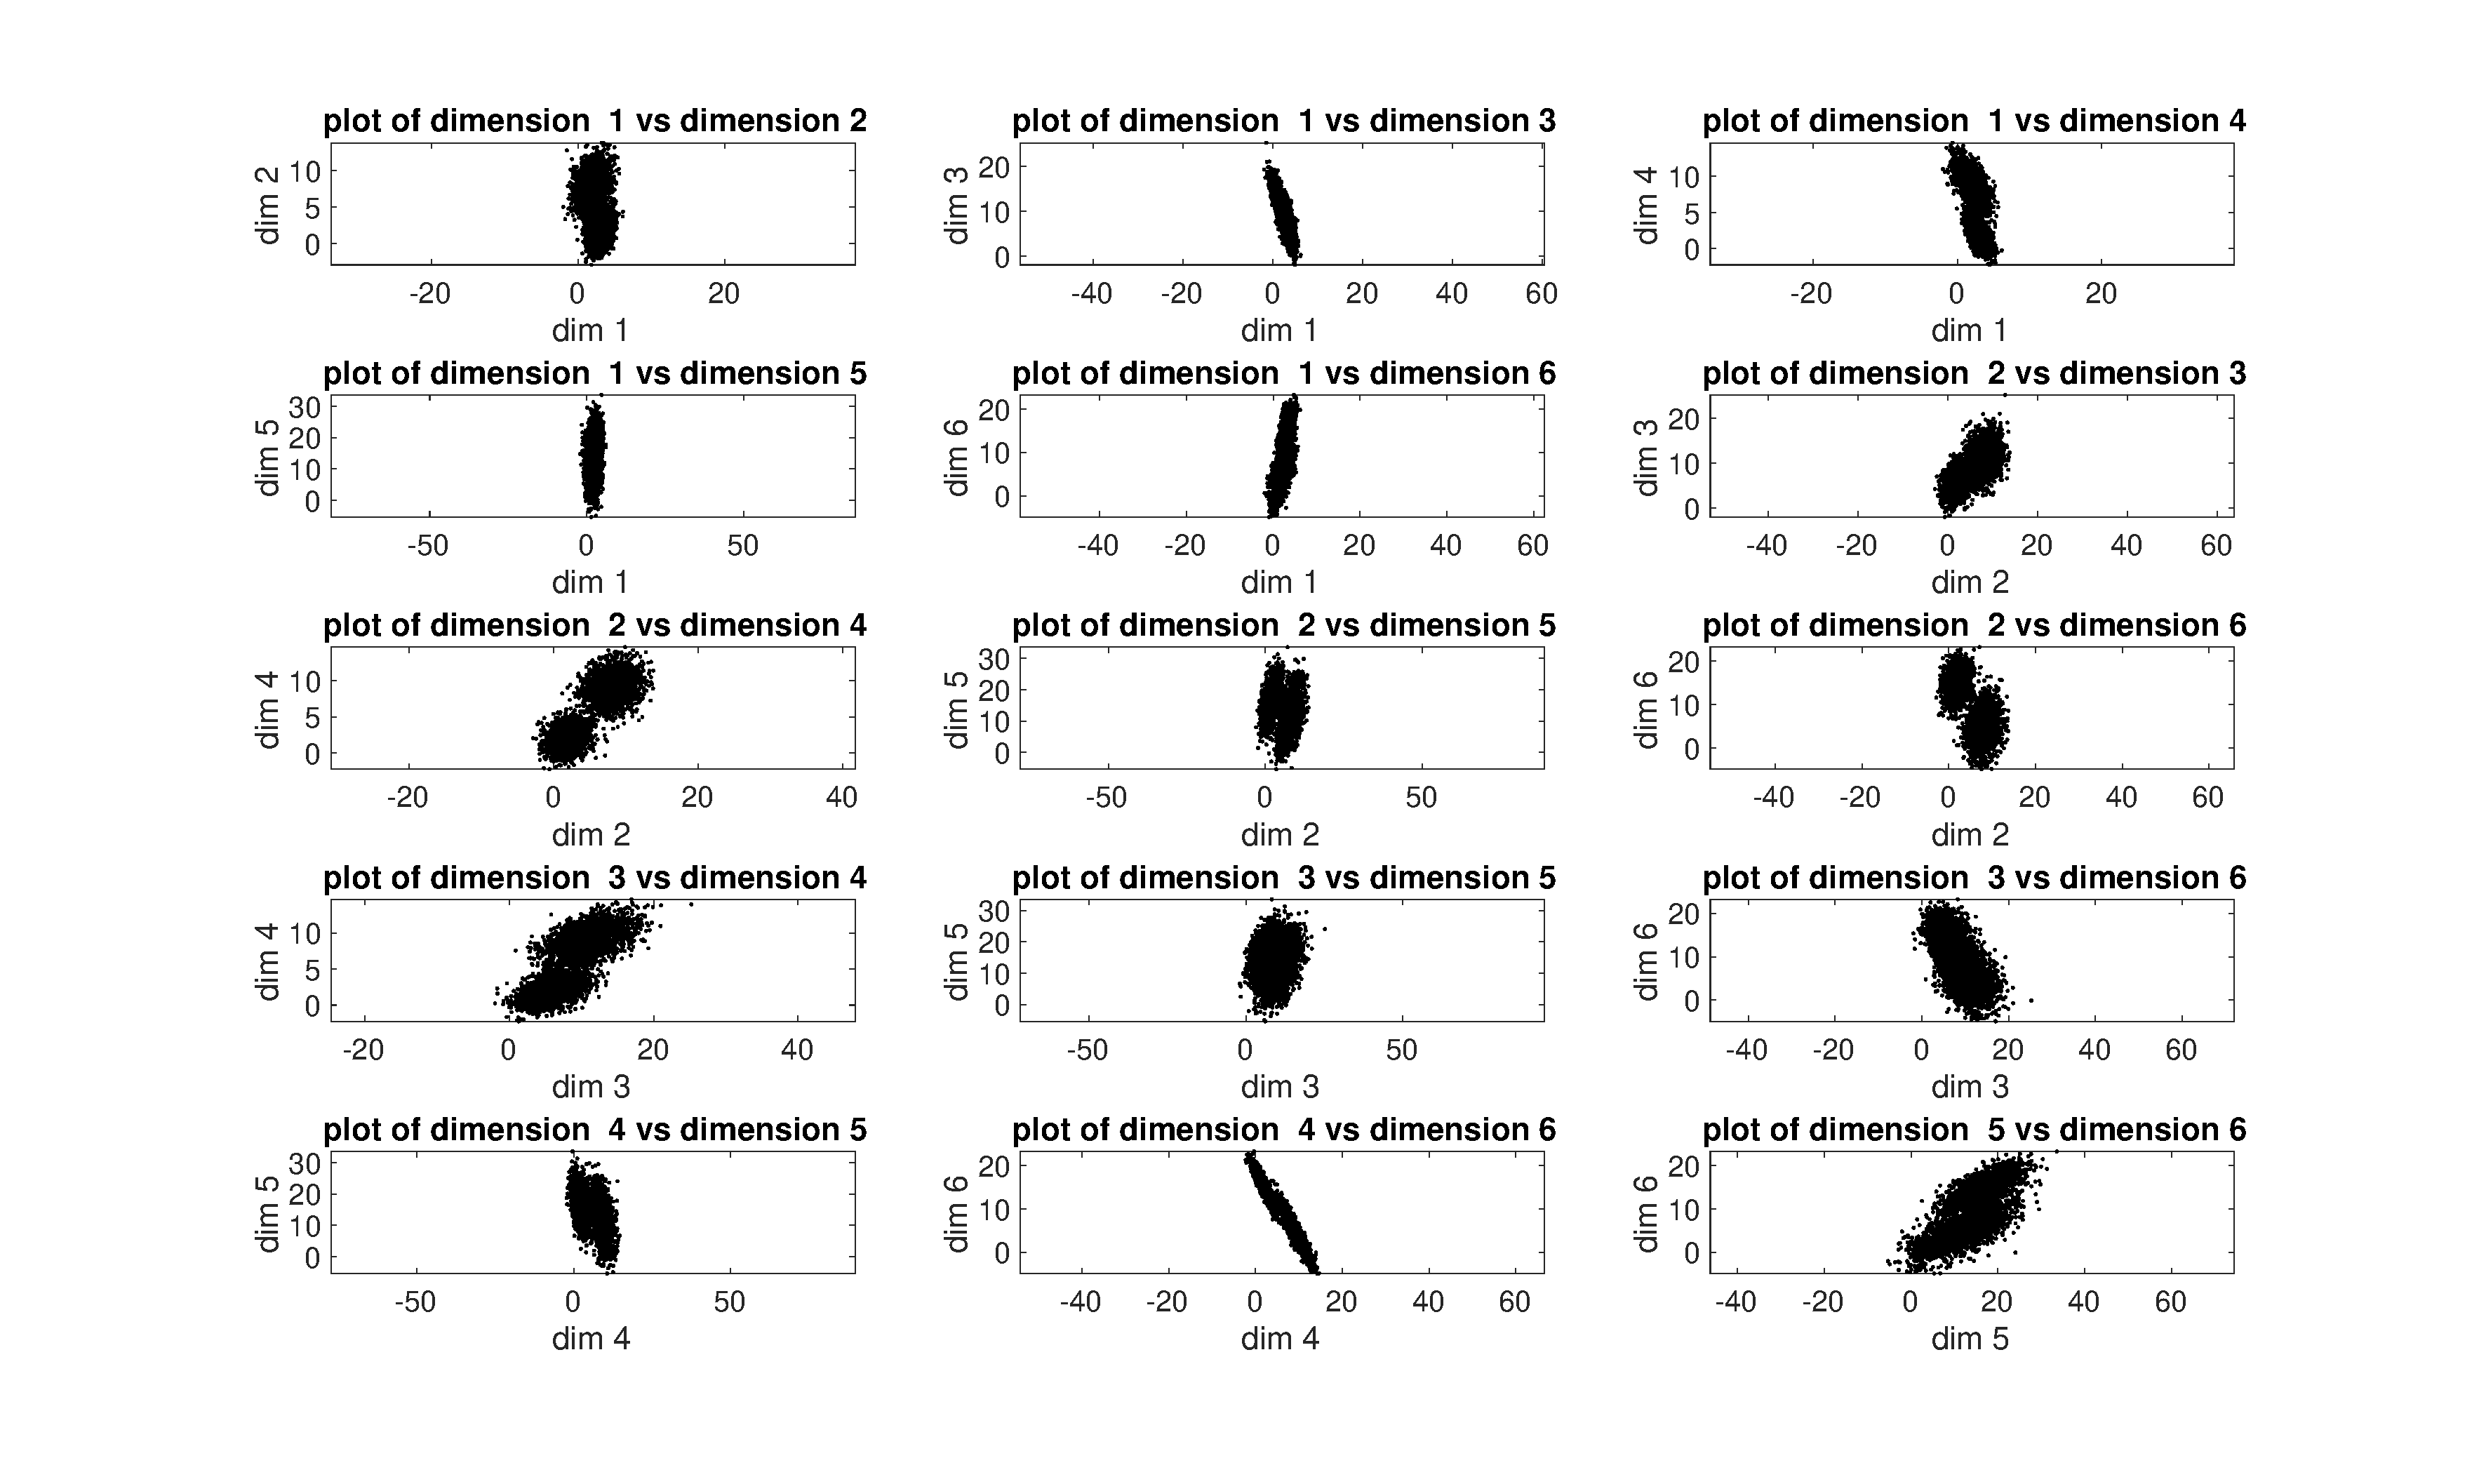
\includegraphics[width=15cm, height=10cm] {Q_1_a_plots}
    }
    \caption{\label{fig:my figure} Scatter plots for every dimension of the data plotted against every other dimension }
\end{figure}

\subsection*{Part (b)}
We are next asked to center the data, compute the SVD, plot the singular values, and plot the first few principal components.  
\begin{itemize}
    \item \textbf{Center the Data}(lines 18-20) \\
    To center the data we first need to know the number of data points in x, so we define [n,p] where n is the number of rows and p the number of columns\\
    We next calculate the mean vector x\_c which contains the mean value of each 6 dimensions by summing over all 6000 entries of X and dividing by 6000 as follows:\\
    \begin{verbatim}19: x_c = (1/p)*sum(X(:,:),2);  \end{verbatim}
    The last step is simply to subtract the x\_c vector from every X data point to center the values about it
    
    \item \textbf{Compute SVD}(line 22) \\
    Trivial in Matlab:
    \begin{verbatim}22: [U,D,V]=svd(X_c, 'econ');    \end{verbatim}
    Doing an 'econ' SVD stops calculating values below the dimensionality of D. Therefore, U is a 6x6 matrix, D is diagonal 6x6 which stores the singular values and V is 4000x6 matrix.  I will refer to these matrices moving forward.
    
    \item \textbf{Plot Singular Values}(lines 24-30) \\
    First, I create a 6x1 singular values vector d by extracting the diagonal of D\\
    Then I plot these 6 values as shown in figure 2.  The plot of singular values shows that the first three are at least one order of magnitude larger than the last 3.  This suggests that the last 3 singular values are less significant and the data can be modeled with 3 dimensions.  \\
    \begin{figure}[h!]
        \centerline
        {
        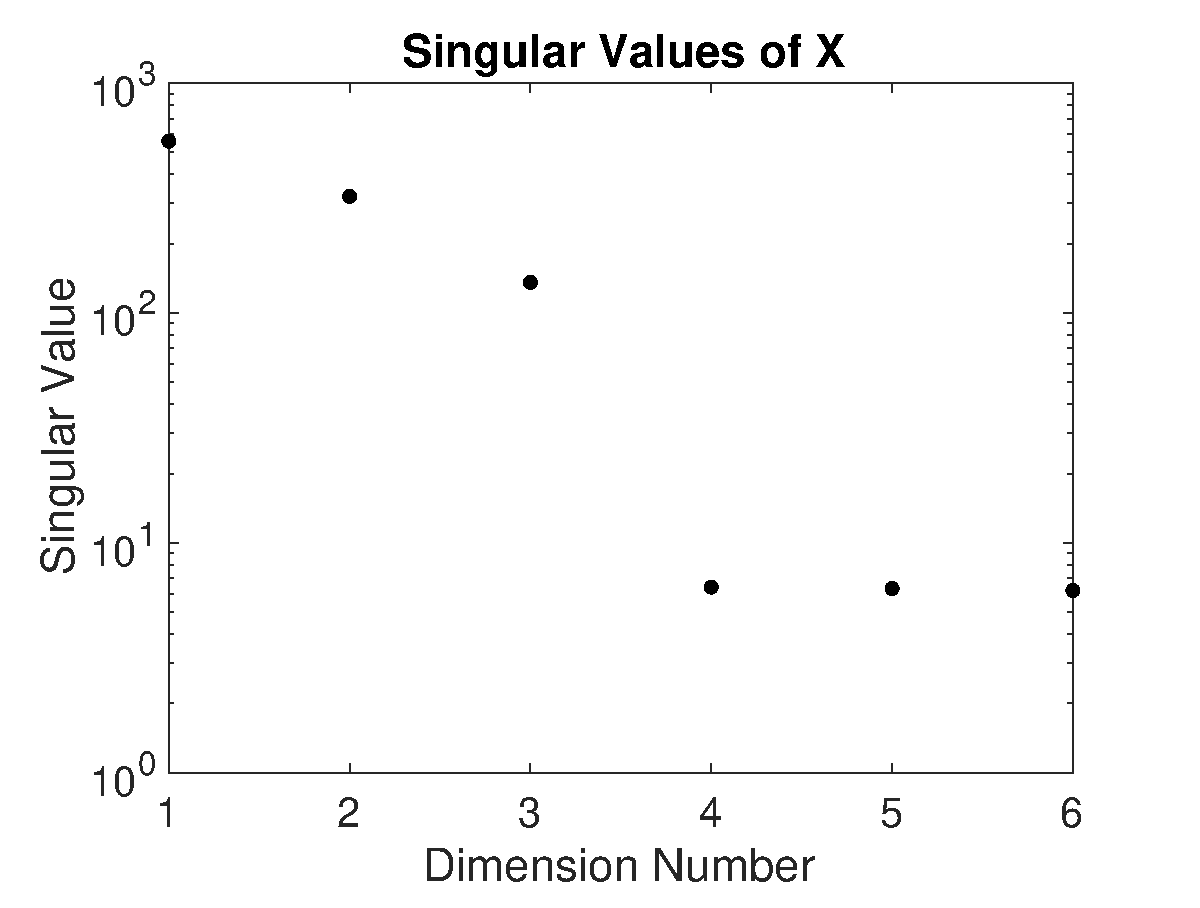
\includegraphics[width=10cm, height=7cm] {Q_1_b_singular_values}
        }
        \caption{\label{fig:my figure} The 6 singular values of the matrix X.  We see that the first 3 values dominate by more than one order of magnitude. }
    \end{figure}

    \item \textbf{Plot Principal Components}(lines 32-70)\\
    The principal components Z of X are mutually orthogonal vectors which decreasingly-effectively approximate the data.  The first k principal components are calculated by multiplying X by the first k feature vectors of (elements of U).  In code I calculated the first principal components by:
    \begin{verbatim}32: Z=U(:,1:3)'*X;\end{verbatim}

    I then plotted all 6 permutations of the principal components in figure (3).  We can see in all graphs including principal component 1 (left square of graphs) a high likelihood for the presence of clusters in the data.  It makes sense that the graphs of 2v3 and 3v2 do not seem as clustered because these principal components reflect the data less strongly than component 1 does.
    \begin{figure}[h!]
        \centerline
        {
        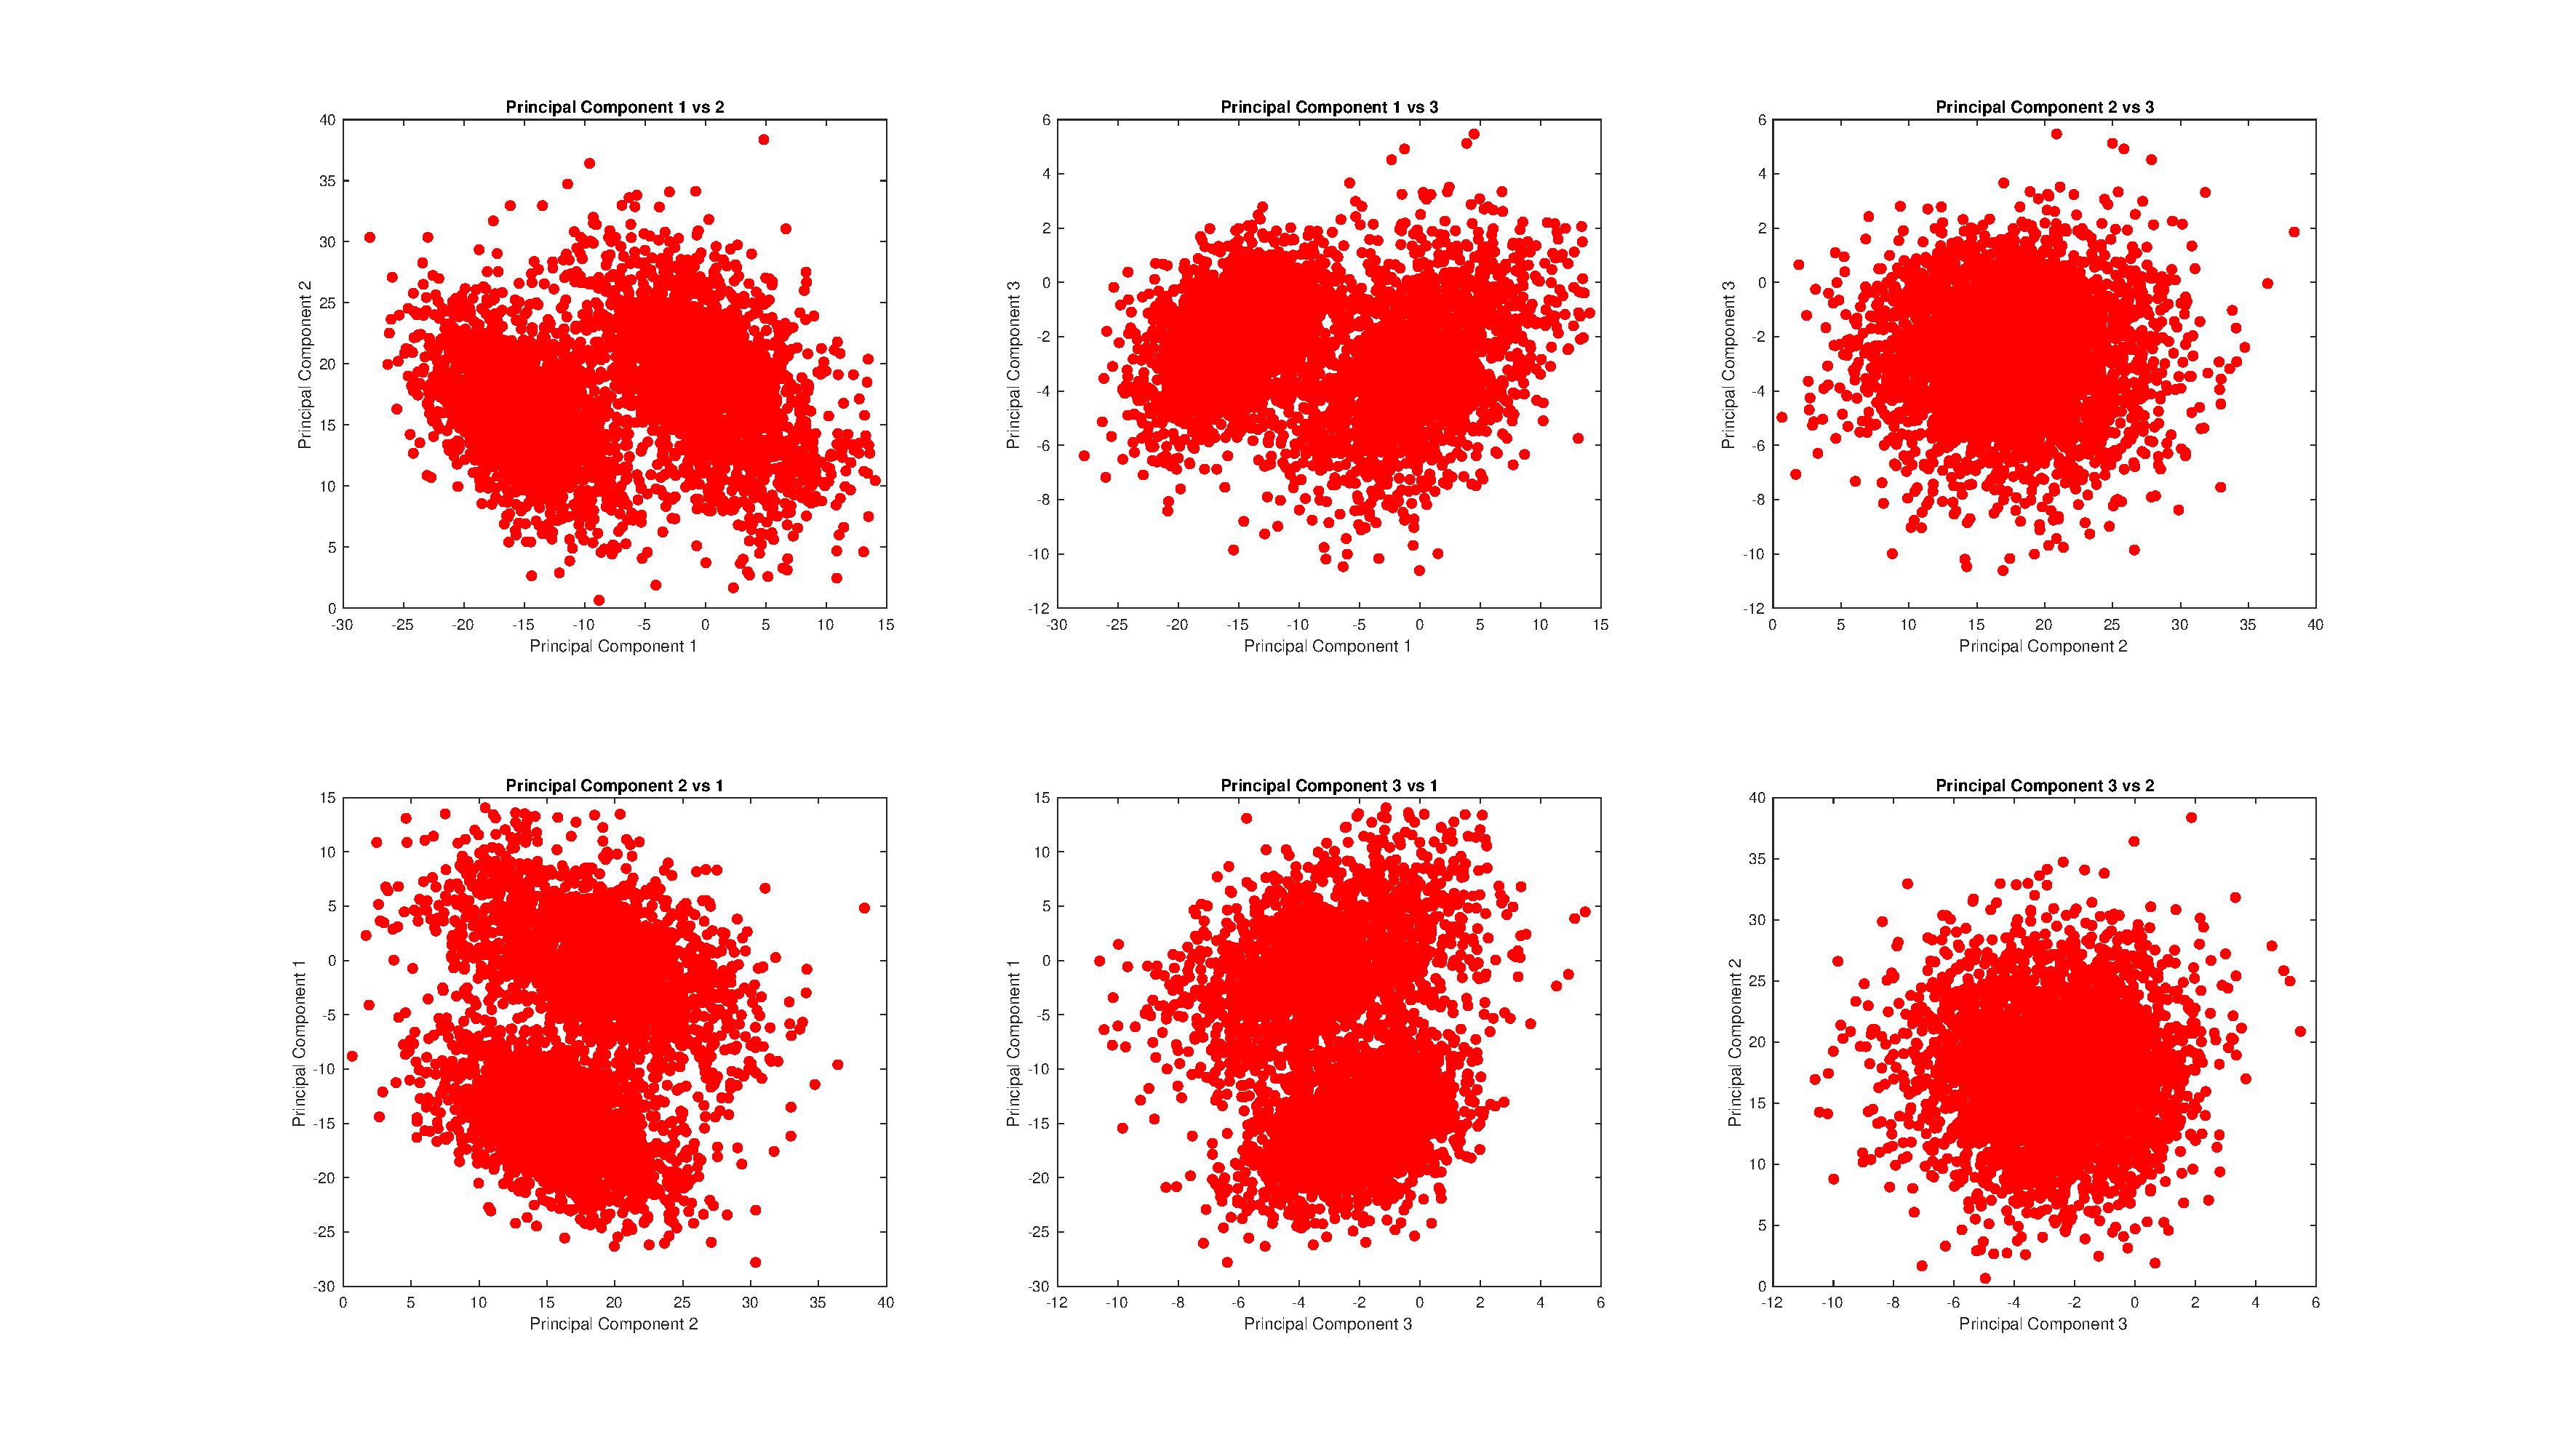
\includegraphics[width=15cm, height=10cm] {Q_1_b_principal_components}
        }
        \caption{\label{fig:my figure} The 6 ways to graph the 3 dominant principal components.  Note the likelihood of ability to cluster data.  Most apparent in the left square of graphs (2v3 doesn't seem to cluster well, likely because they are less representative of the data set) }
    \end{figure}
\end{itemize}
\pagebreak

\pagebreak
\section*{Problem 2}

\subsection*{Overview}
This problem asks to analyze the file 'HandwritenDigits.mat.'  This file contains matrix X (256x1707) which contains pixel images of 1707 handwritten digits.  There is also annotation vector I which indicates which digit each image represents. All analysis for this problem will be on the data corresponding to the first 5 images for digits 0, 1, 3, and 7. \\
We are tasked to approximate the samples as the linear combination of different numbers of feature vectors.  Then we plot these approximation images and their residuals.  Lastly we plot the norms and errors as a function of the number of feature vectors.  

\subsection*{Approximation via Linear Combination of Feature Vectors}
As we defined above, the principal component matrix Z=U'X.   We can see that by substituting X=UDV' we can rewrite as a Z=DV'.  Therefore,  we can solve for X=UZ.  Z is a matrix of vectors corresponding to the k-th principal components.  We can therefore approximate X as the linear combination of the first k components as follows:
        \[x^{(j)}\approx P_k x^{(j)} = \sum_{l=1}^{k} z_{l}^{(j)} u^{(l)}\]
        
It is obvious to see that when k = the number of components (256 here) this linear combination returns the complete image, not an approximation.\\
We will approximate the samples as a linear combination of the first k=[5,10,15,20,25] feature vectors.  My analysis will be for images corresponding to 0 but the methodology is identical for 1, 3, and 7\\
I make a nested for loop, the outer loop iterating from i=1:5 (to analyze all 5 samples) and the inner loop iterating from k=1:5 (k represents the feature vectors so I multiply by 5 to yield 5,10,etc...).  
\\I calculate z given the first k feature vectors as:
\begin{verbatim}8: z = U(:,1:5*k)'*X_0(:,i);\end{verbatim}
which directly follows from the math above.  The X\_0 matrix is a subset of X for all images corresponding to 0.  Next, we find the approximation of the image by following the above math as: 
\begin{verbatim}9: reconstructed_x_0 = U(:,1:5*k)*z;\end{verbatim}
Lastly, I find the residual, or the difference from the image and approximation, as follows:
\begin{verbatim}10: this_residual_0 = X_0(:,i)-reconstructed_x_0;
\end{verbatim}

\subsection*{Plot Approximations and Residuals}
    \begin{figure}[!h]
        \centerline
        {
        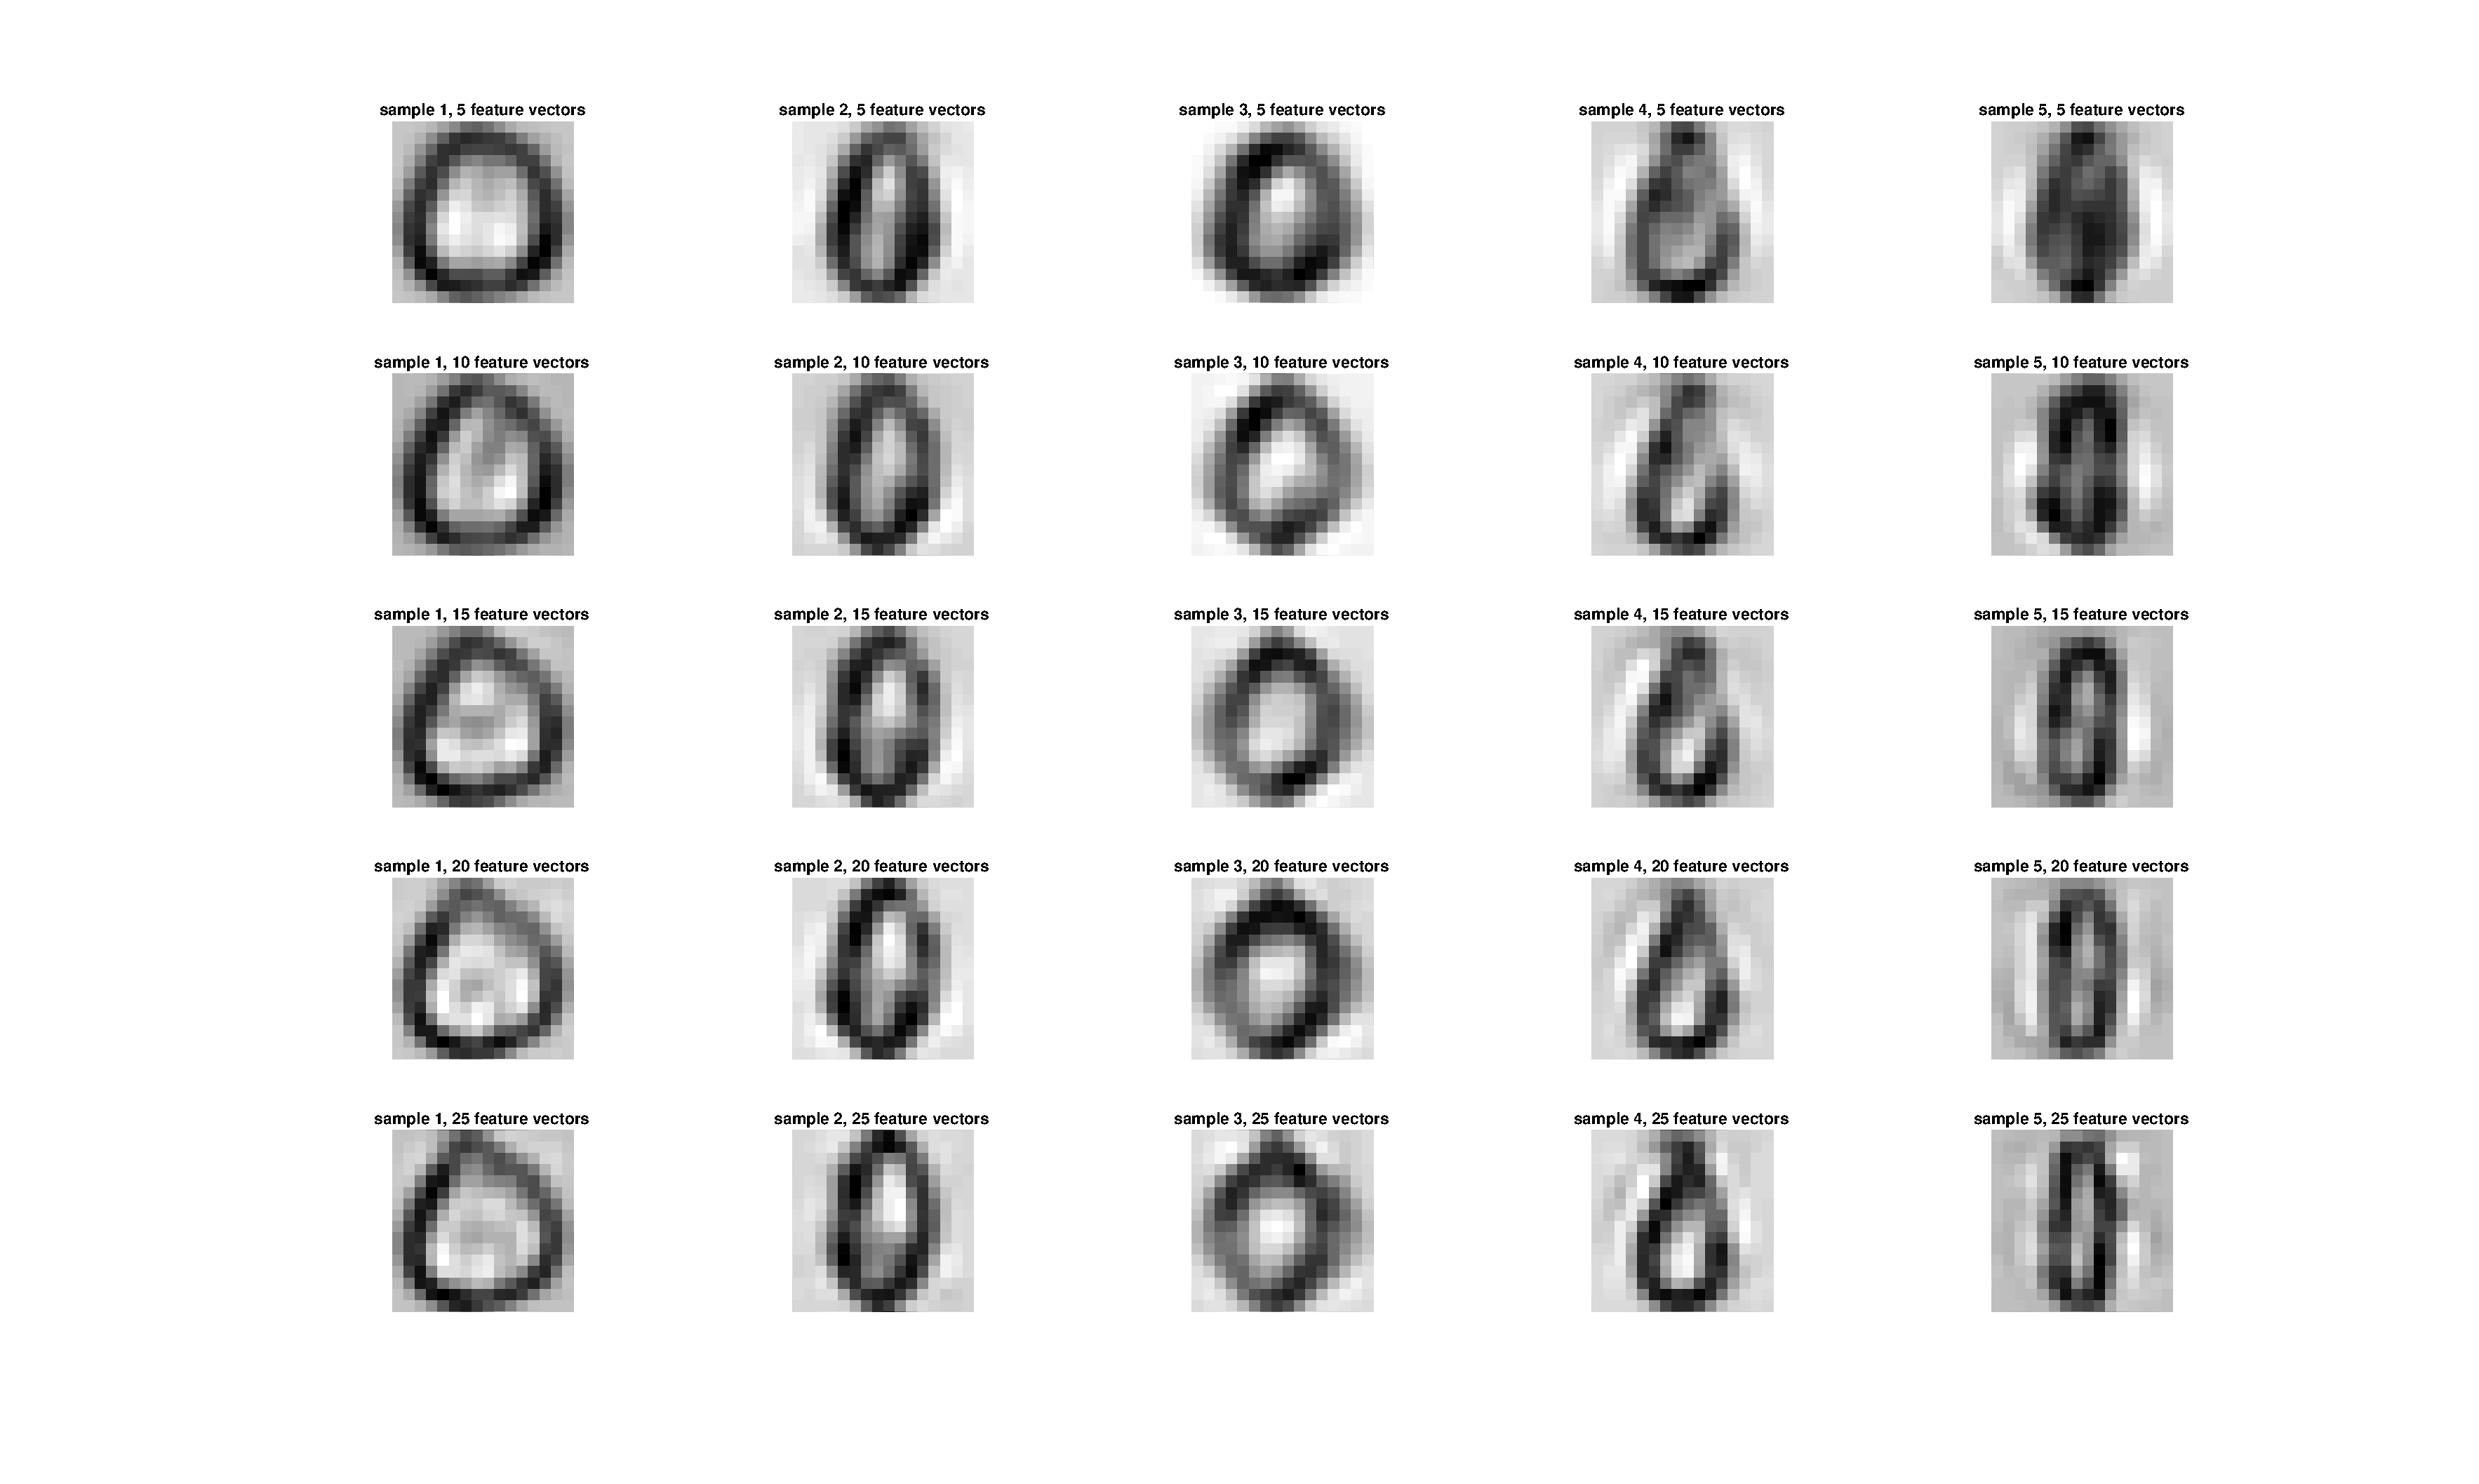
\includegraphics[width=10cm, height=8cm] {Q_2_0_approx}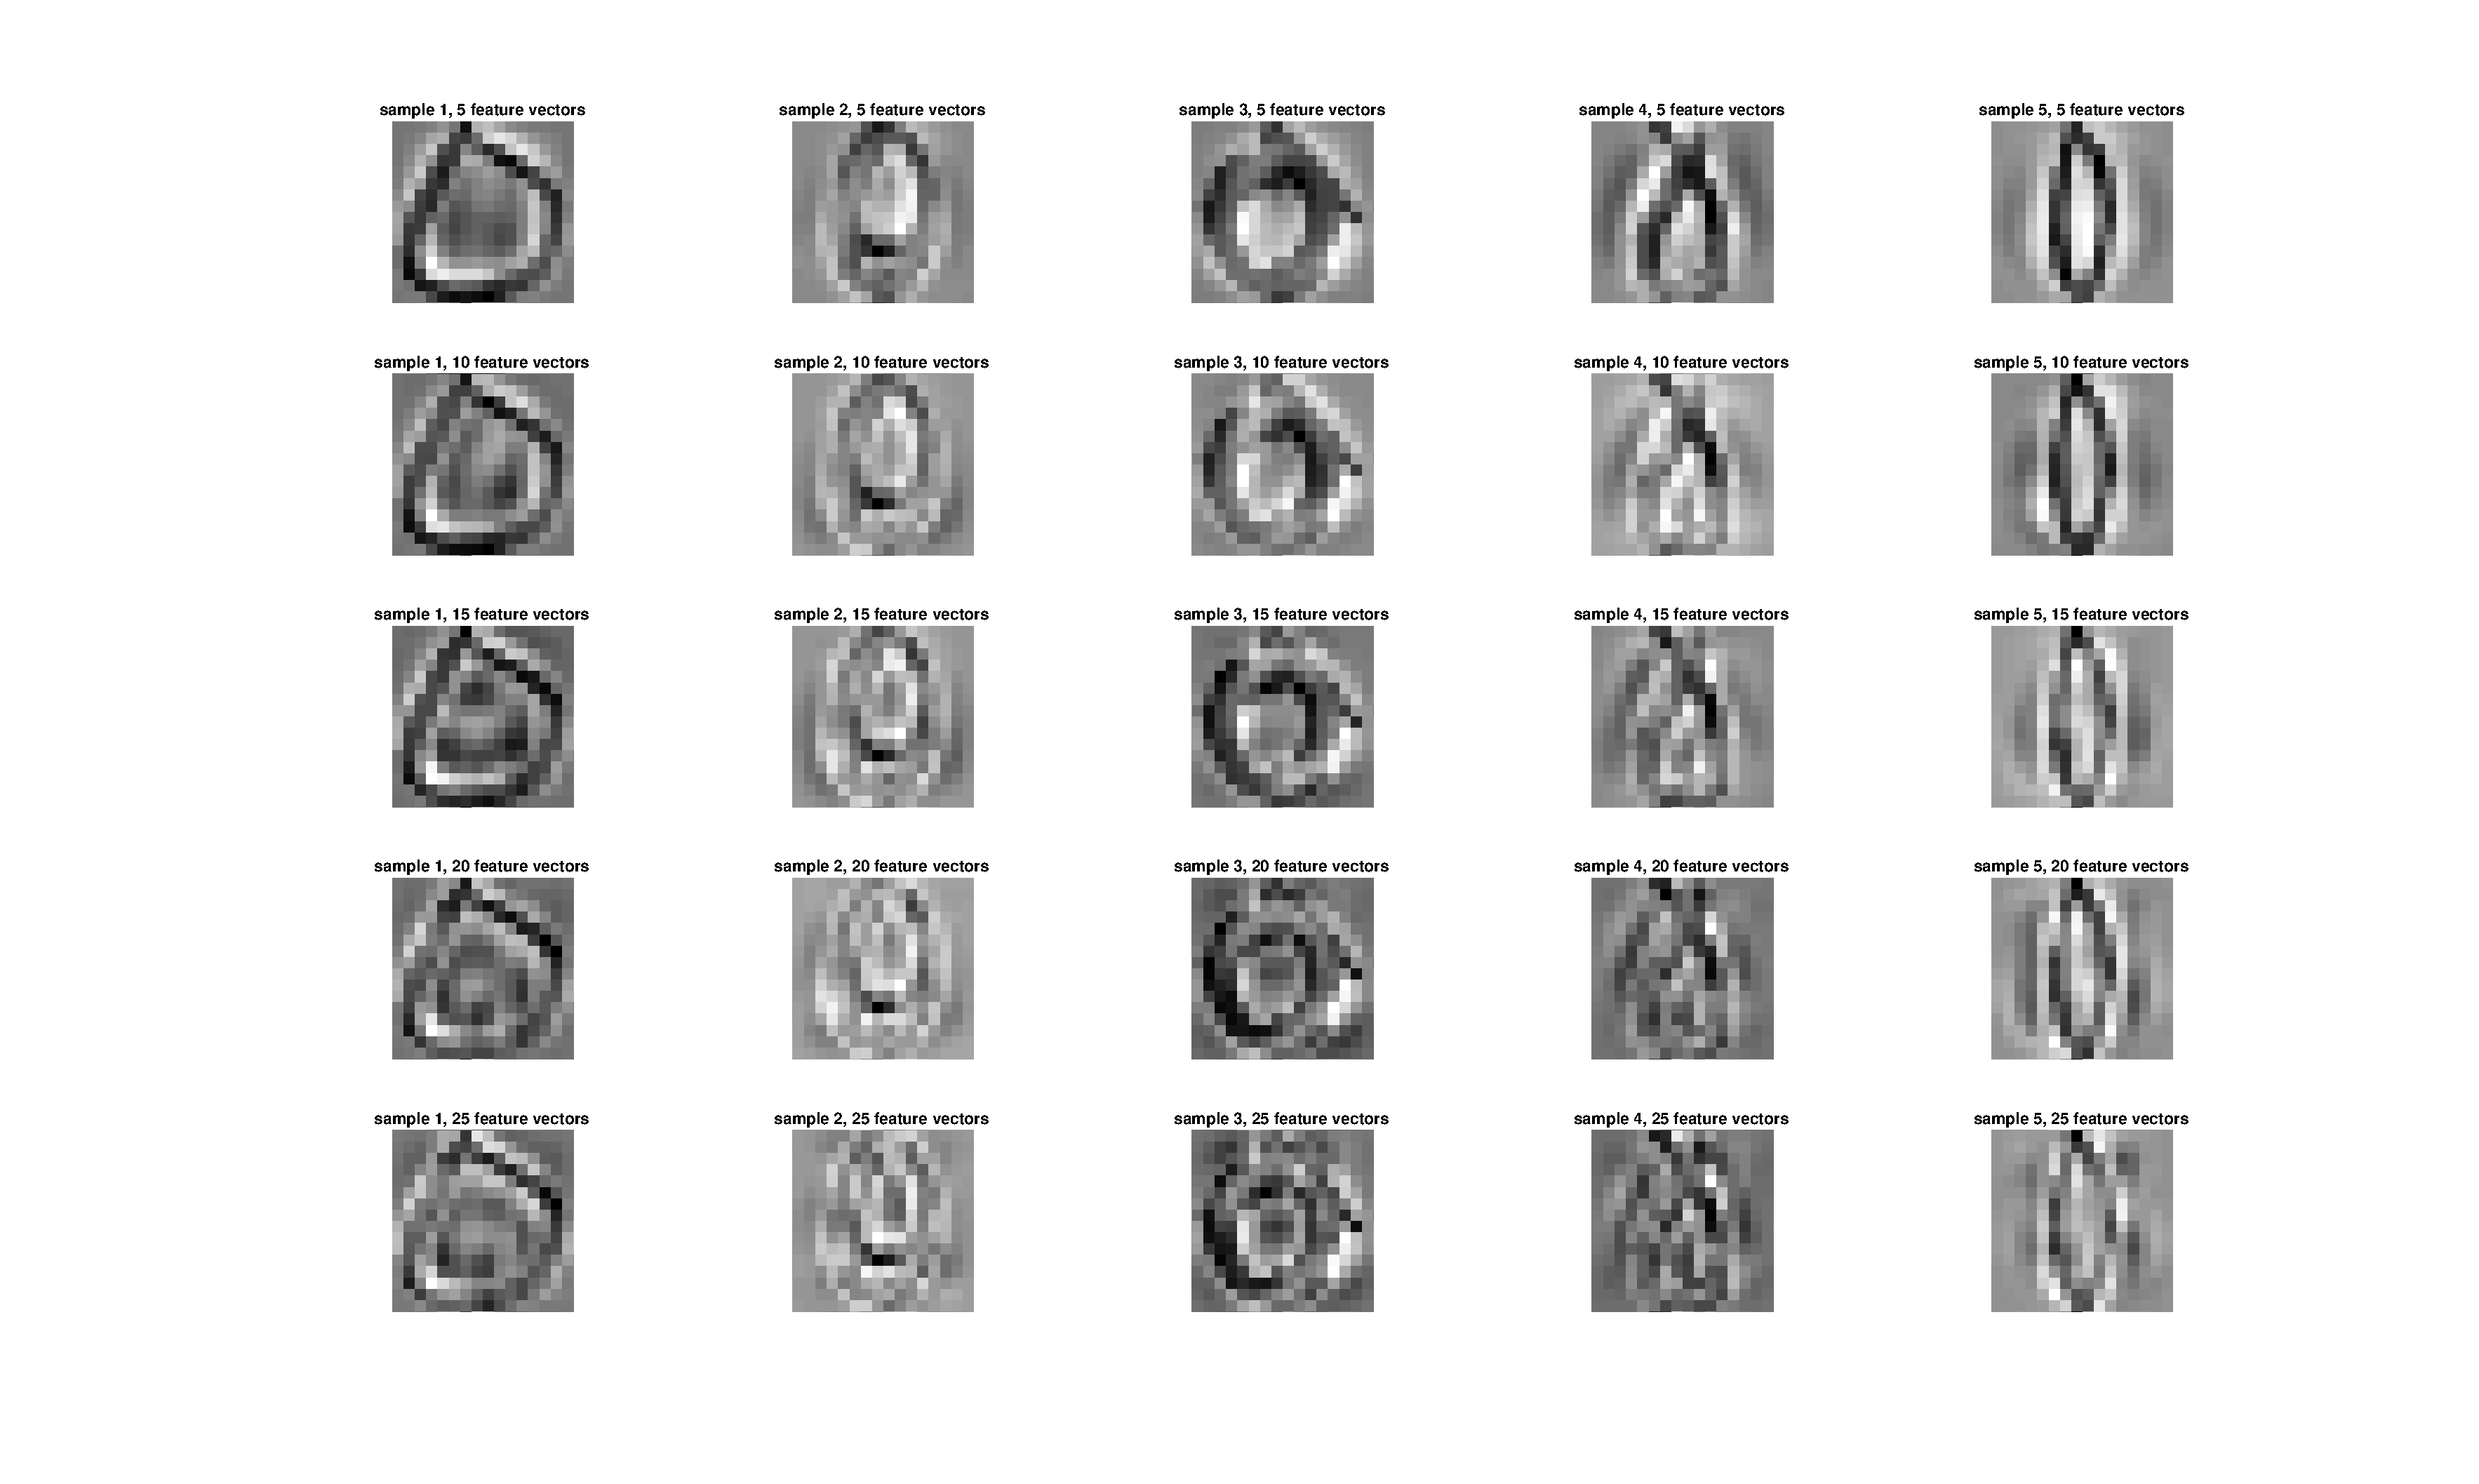
\includegraphics[width=10cm, height=8cm]{Q_2_0_residual}
        }
        \caption{\label{fig:my figure}  In the left panel the approximation of 5 samples of digit 0 using an increasing number of feature vectors.  Each column is a sample image, and the number of feature vectors increases from k=5:25 moving down the column.  The right panel shows the residuals in the same fashion.}
    \end{figure}
    
    \begin{figure}[!h]
        \centerline
        {
        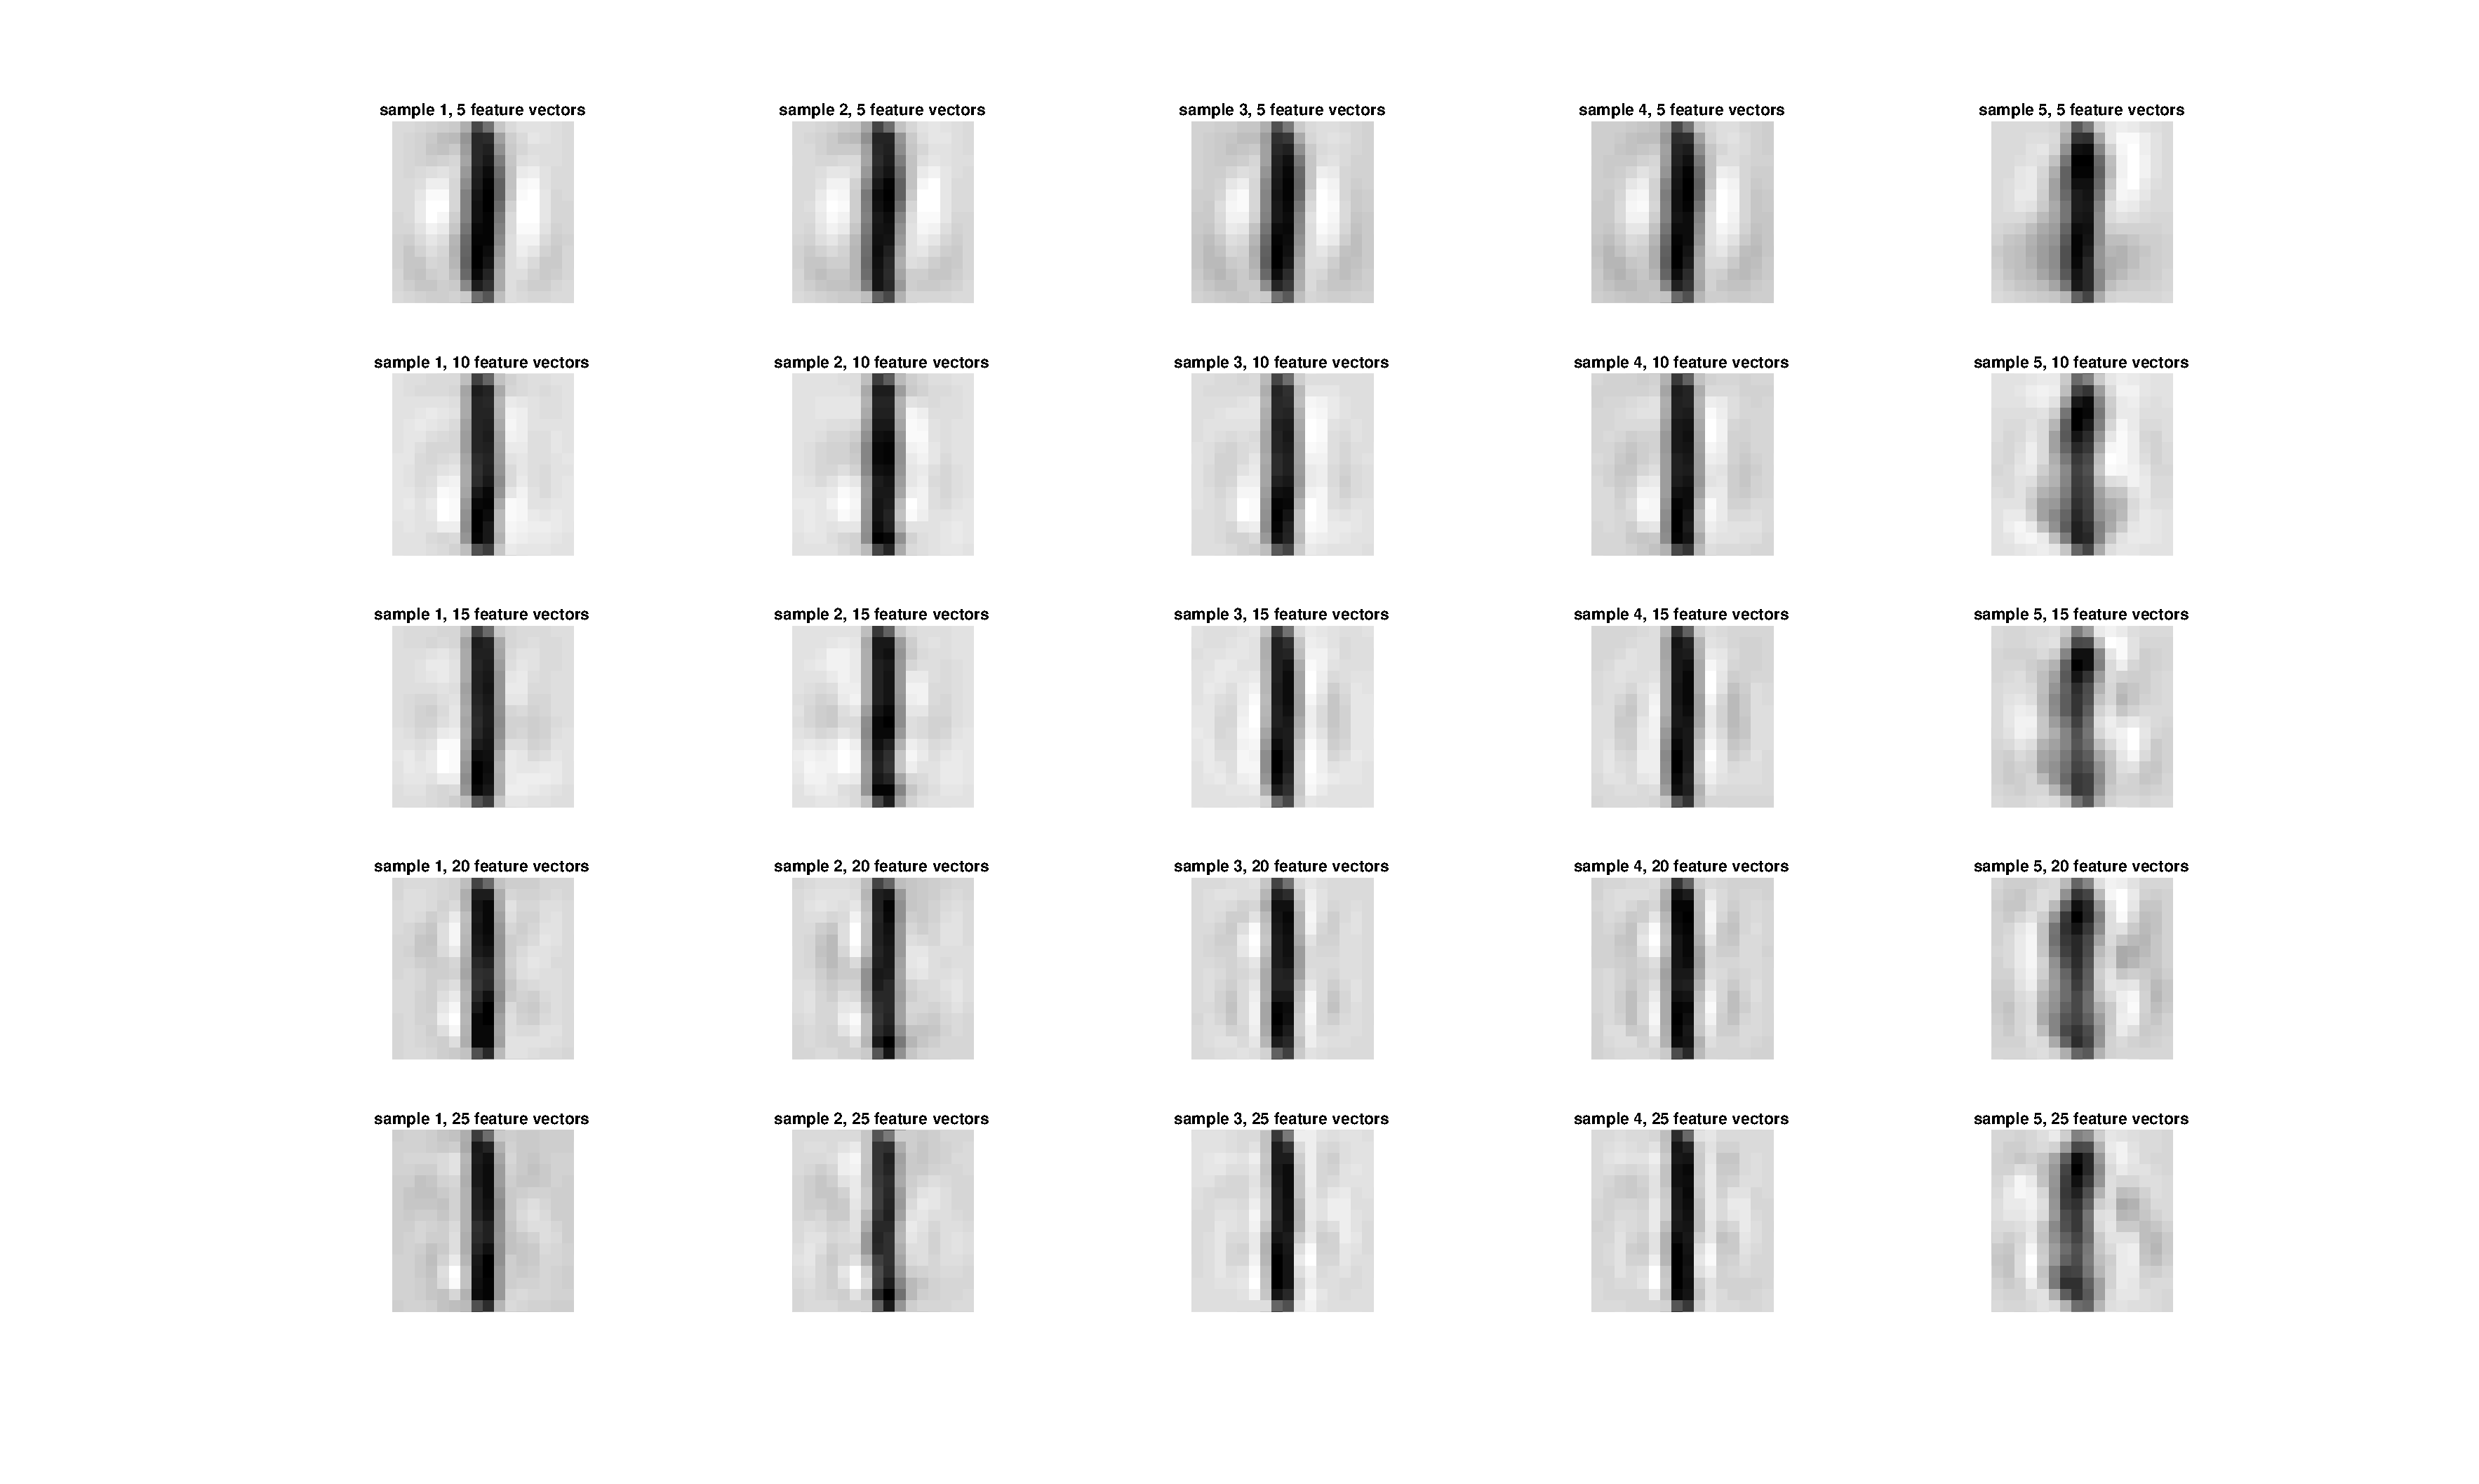
\includegraphics[width=10cm, height=8cm] {Q_2_1_approx}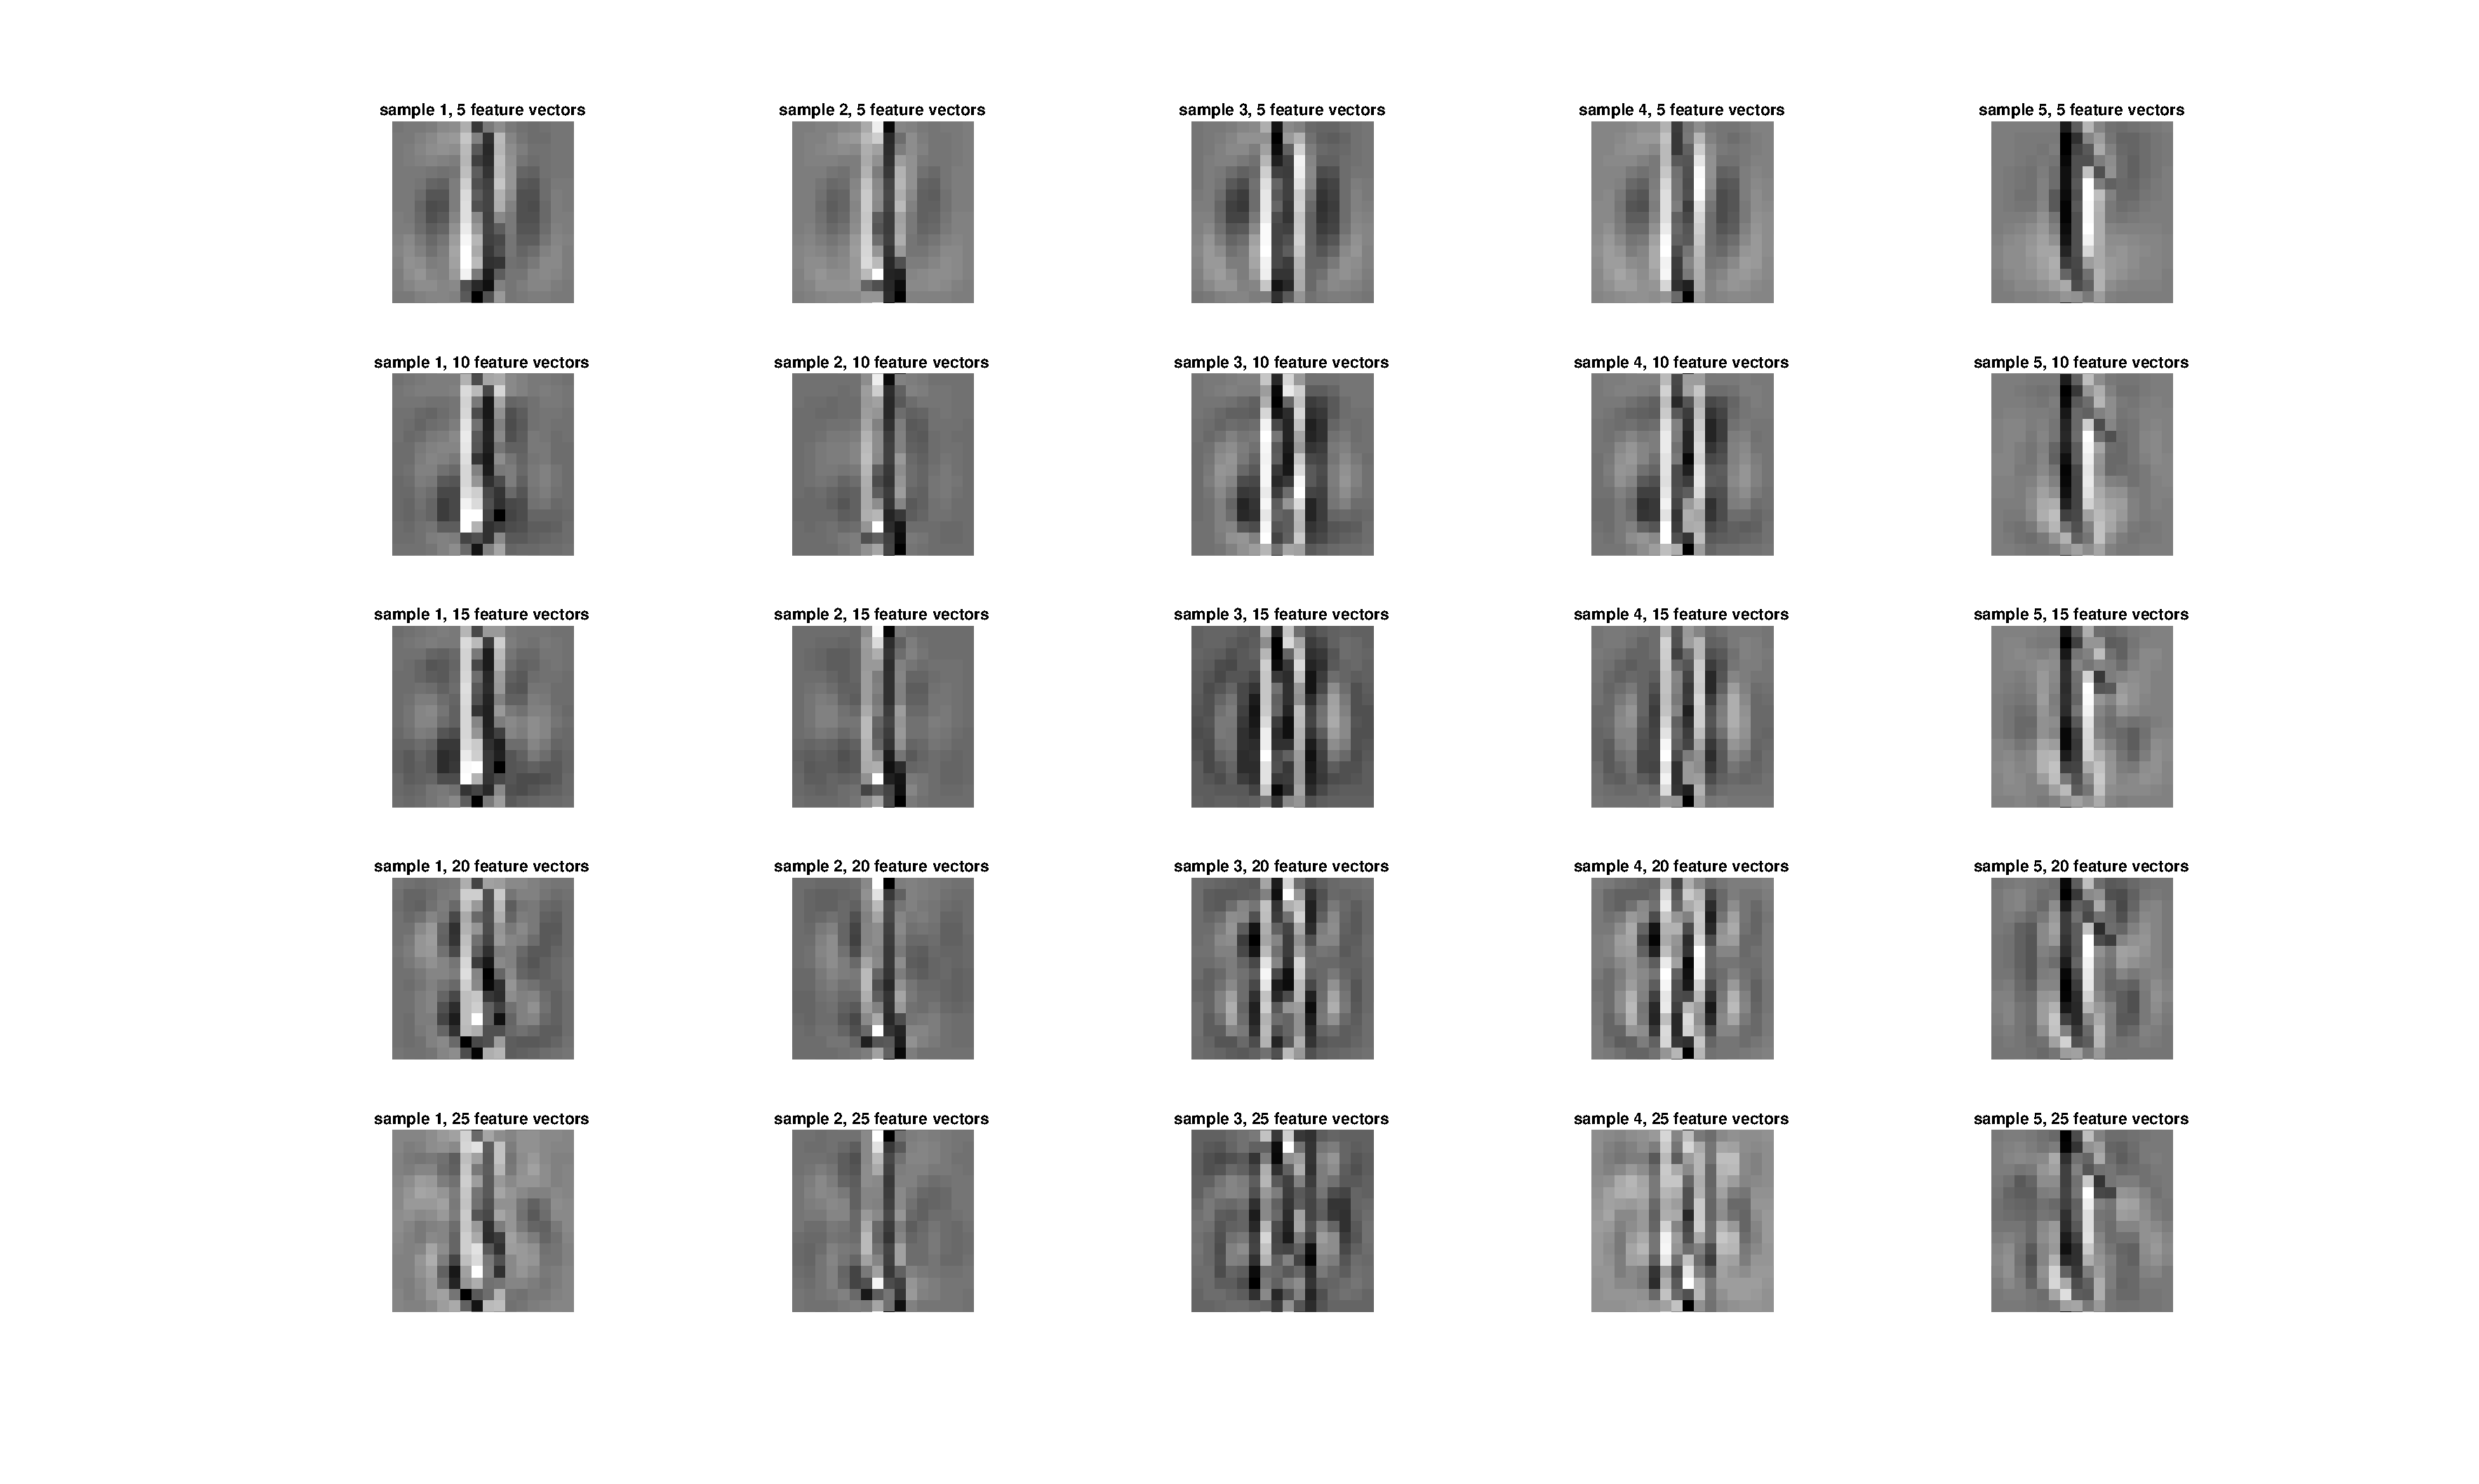
\includegraphics[width=10cm, height=8cm]{Q_2_1_residual}
        }
        \caption{\label{fig:my figure} In the left panel the approximation of 5 samples of digit 1 using an increasing number of feature vectors.  Each column is a sample image, and the number of feature vectors increases from k=5:25 moving down the column.  The right panel shows the residuals in the same fashion.}
    \end{figure}
    
    \begin{figure}[!h]
        \centerline
        {
        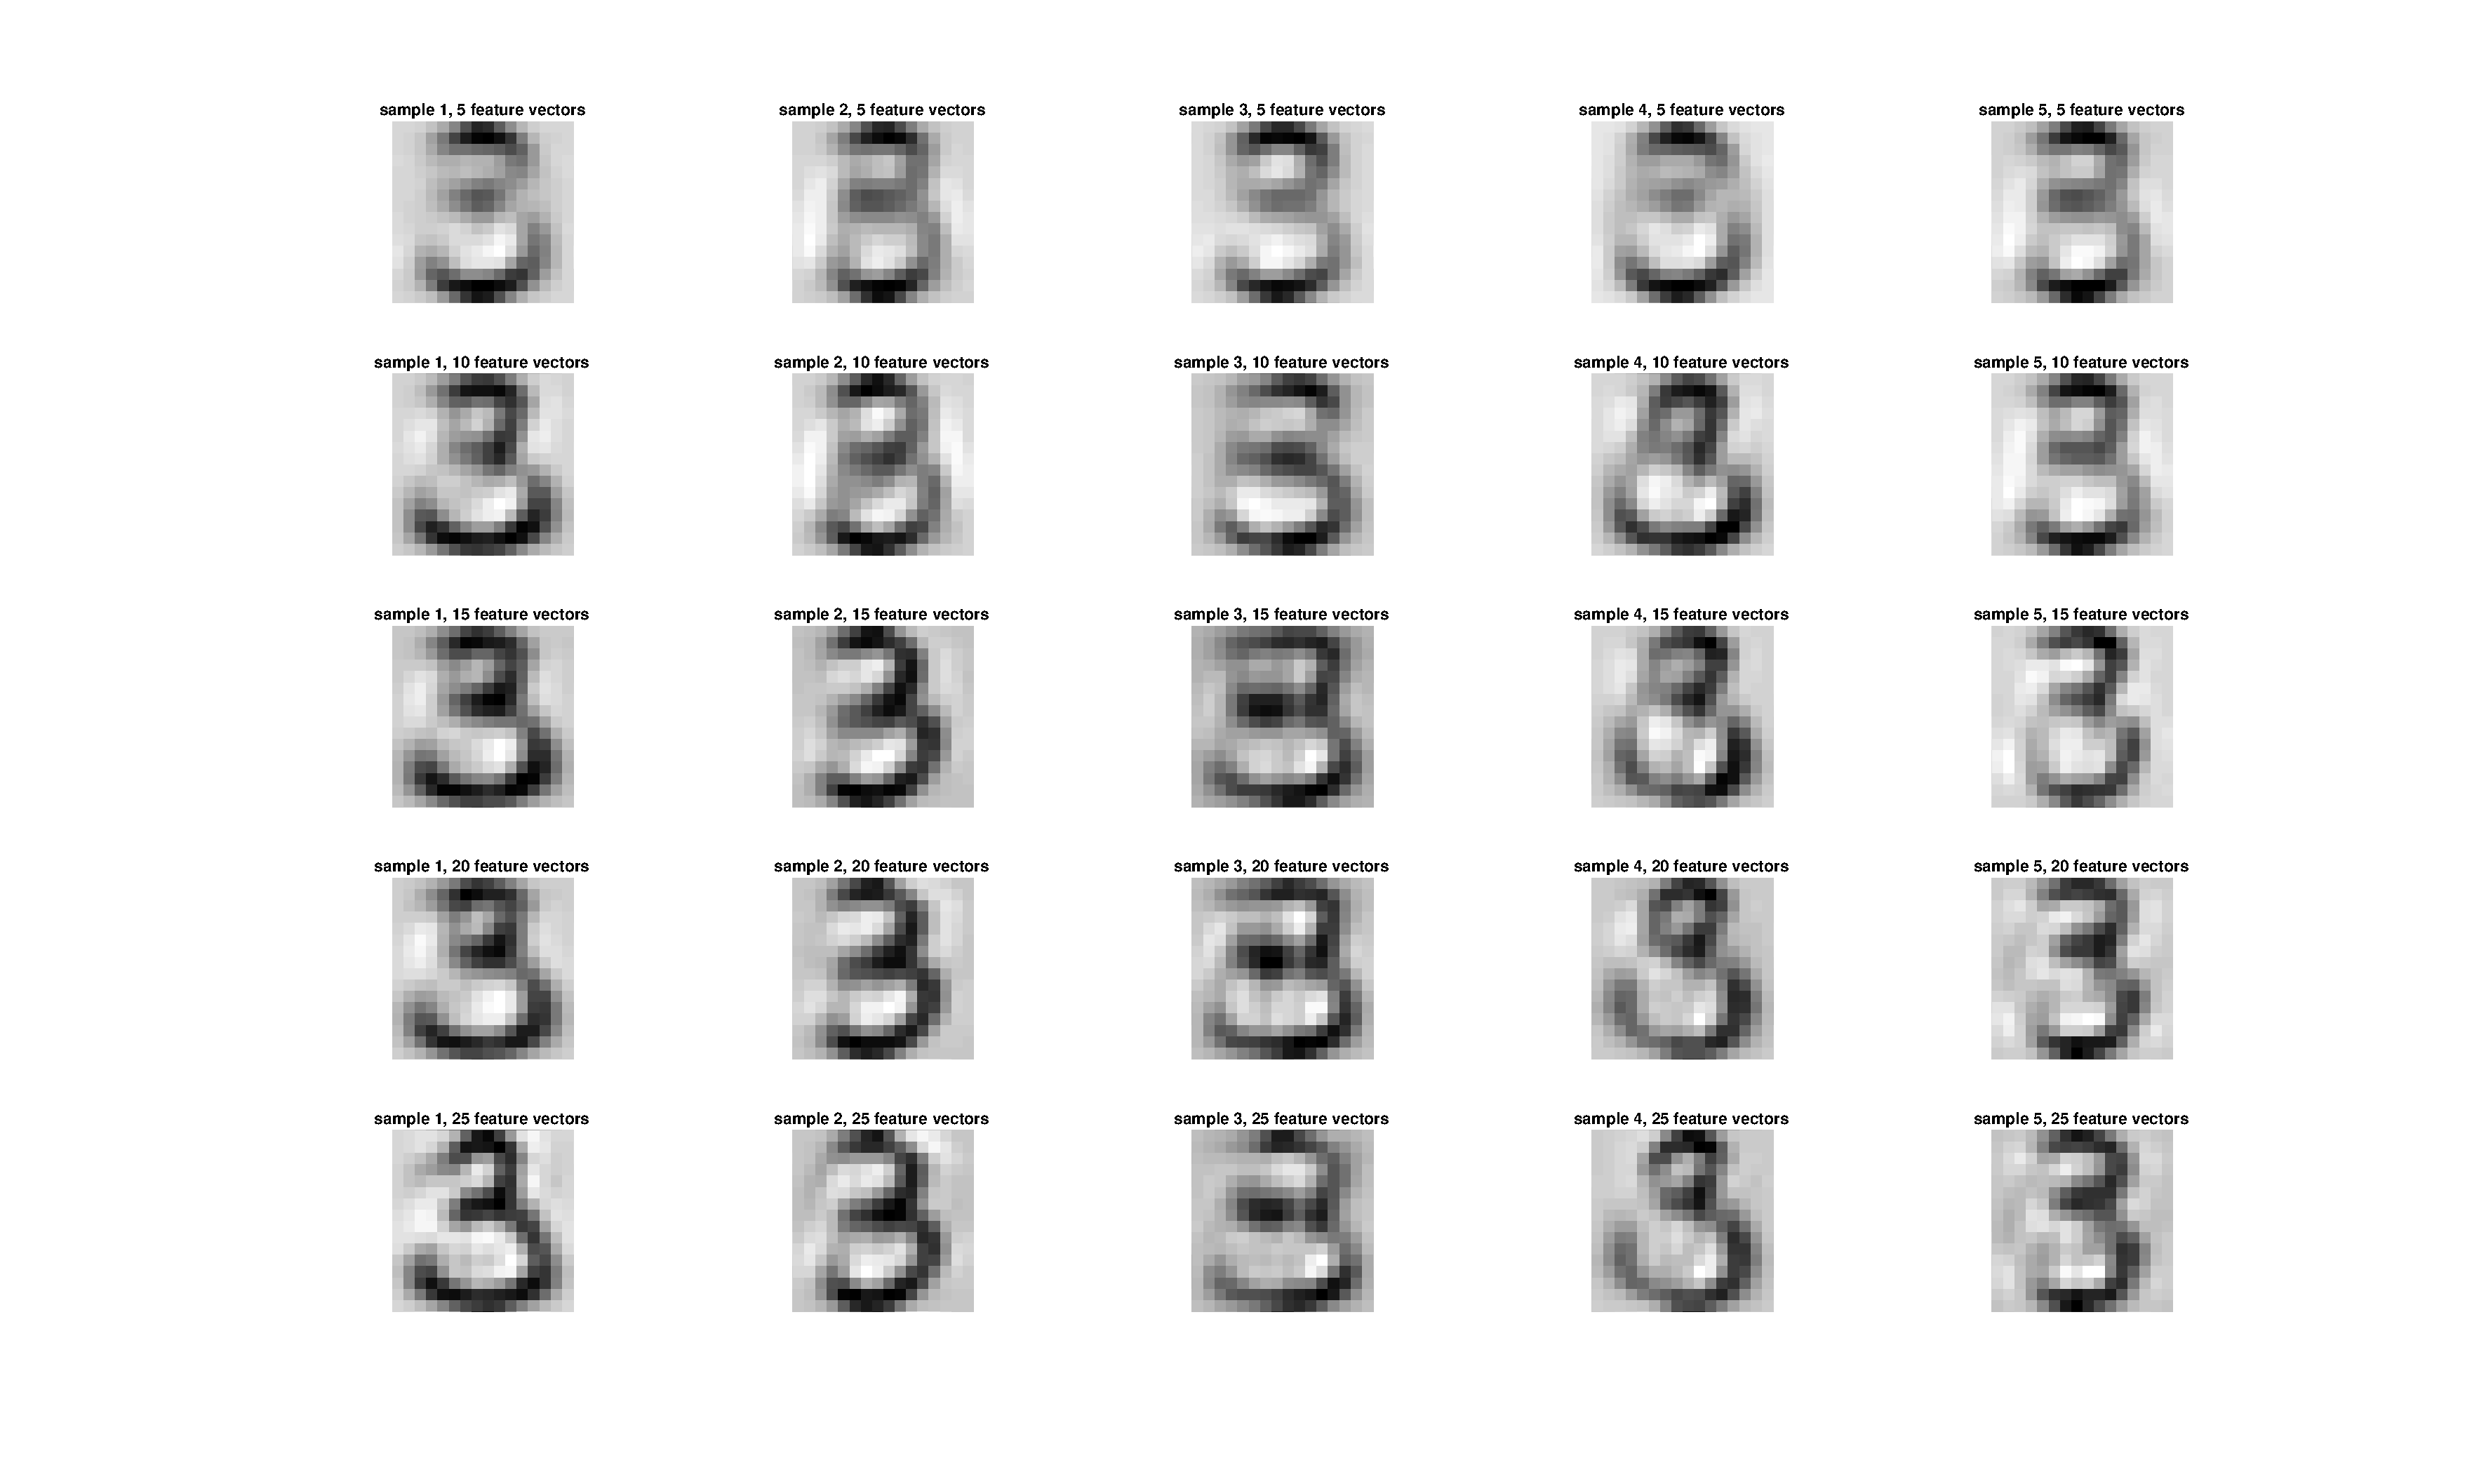
\includegraphics[width=10cm, height=8cm] {Q_2_3_approx}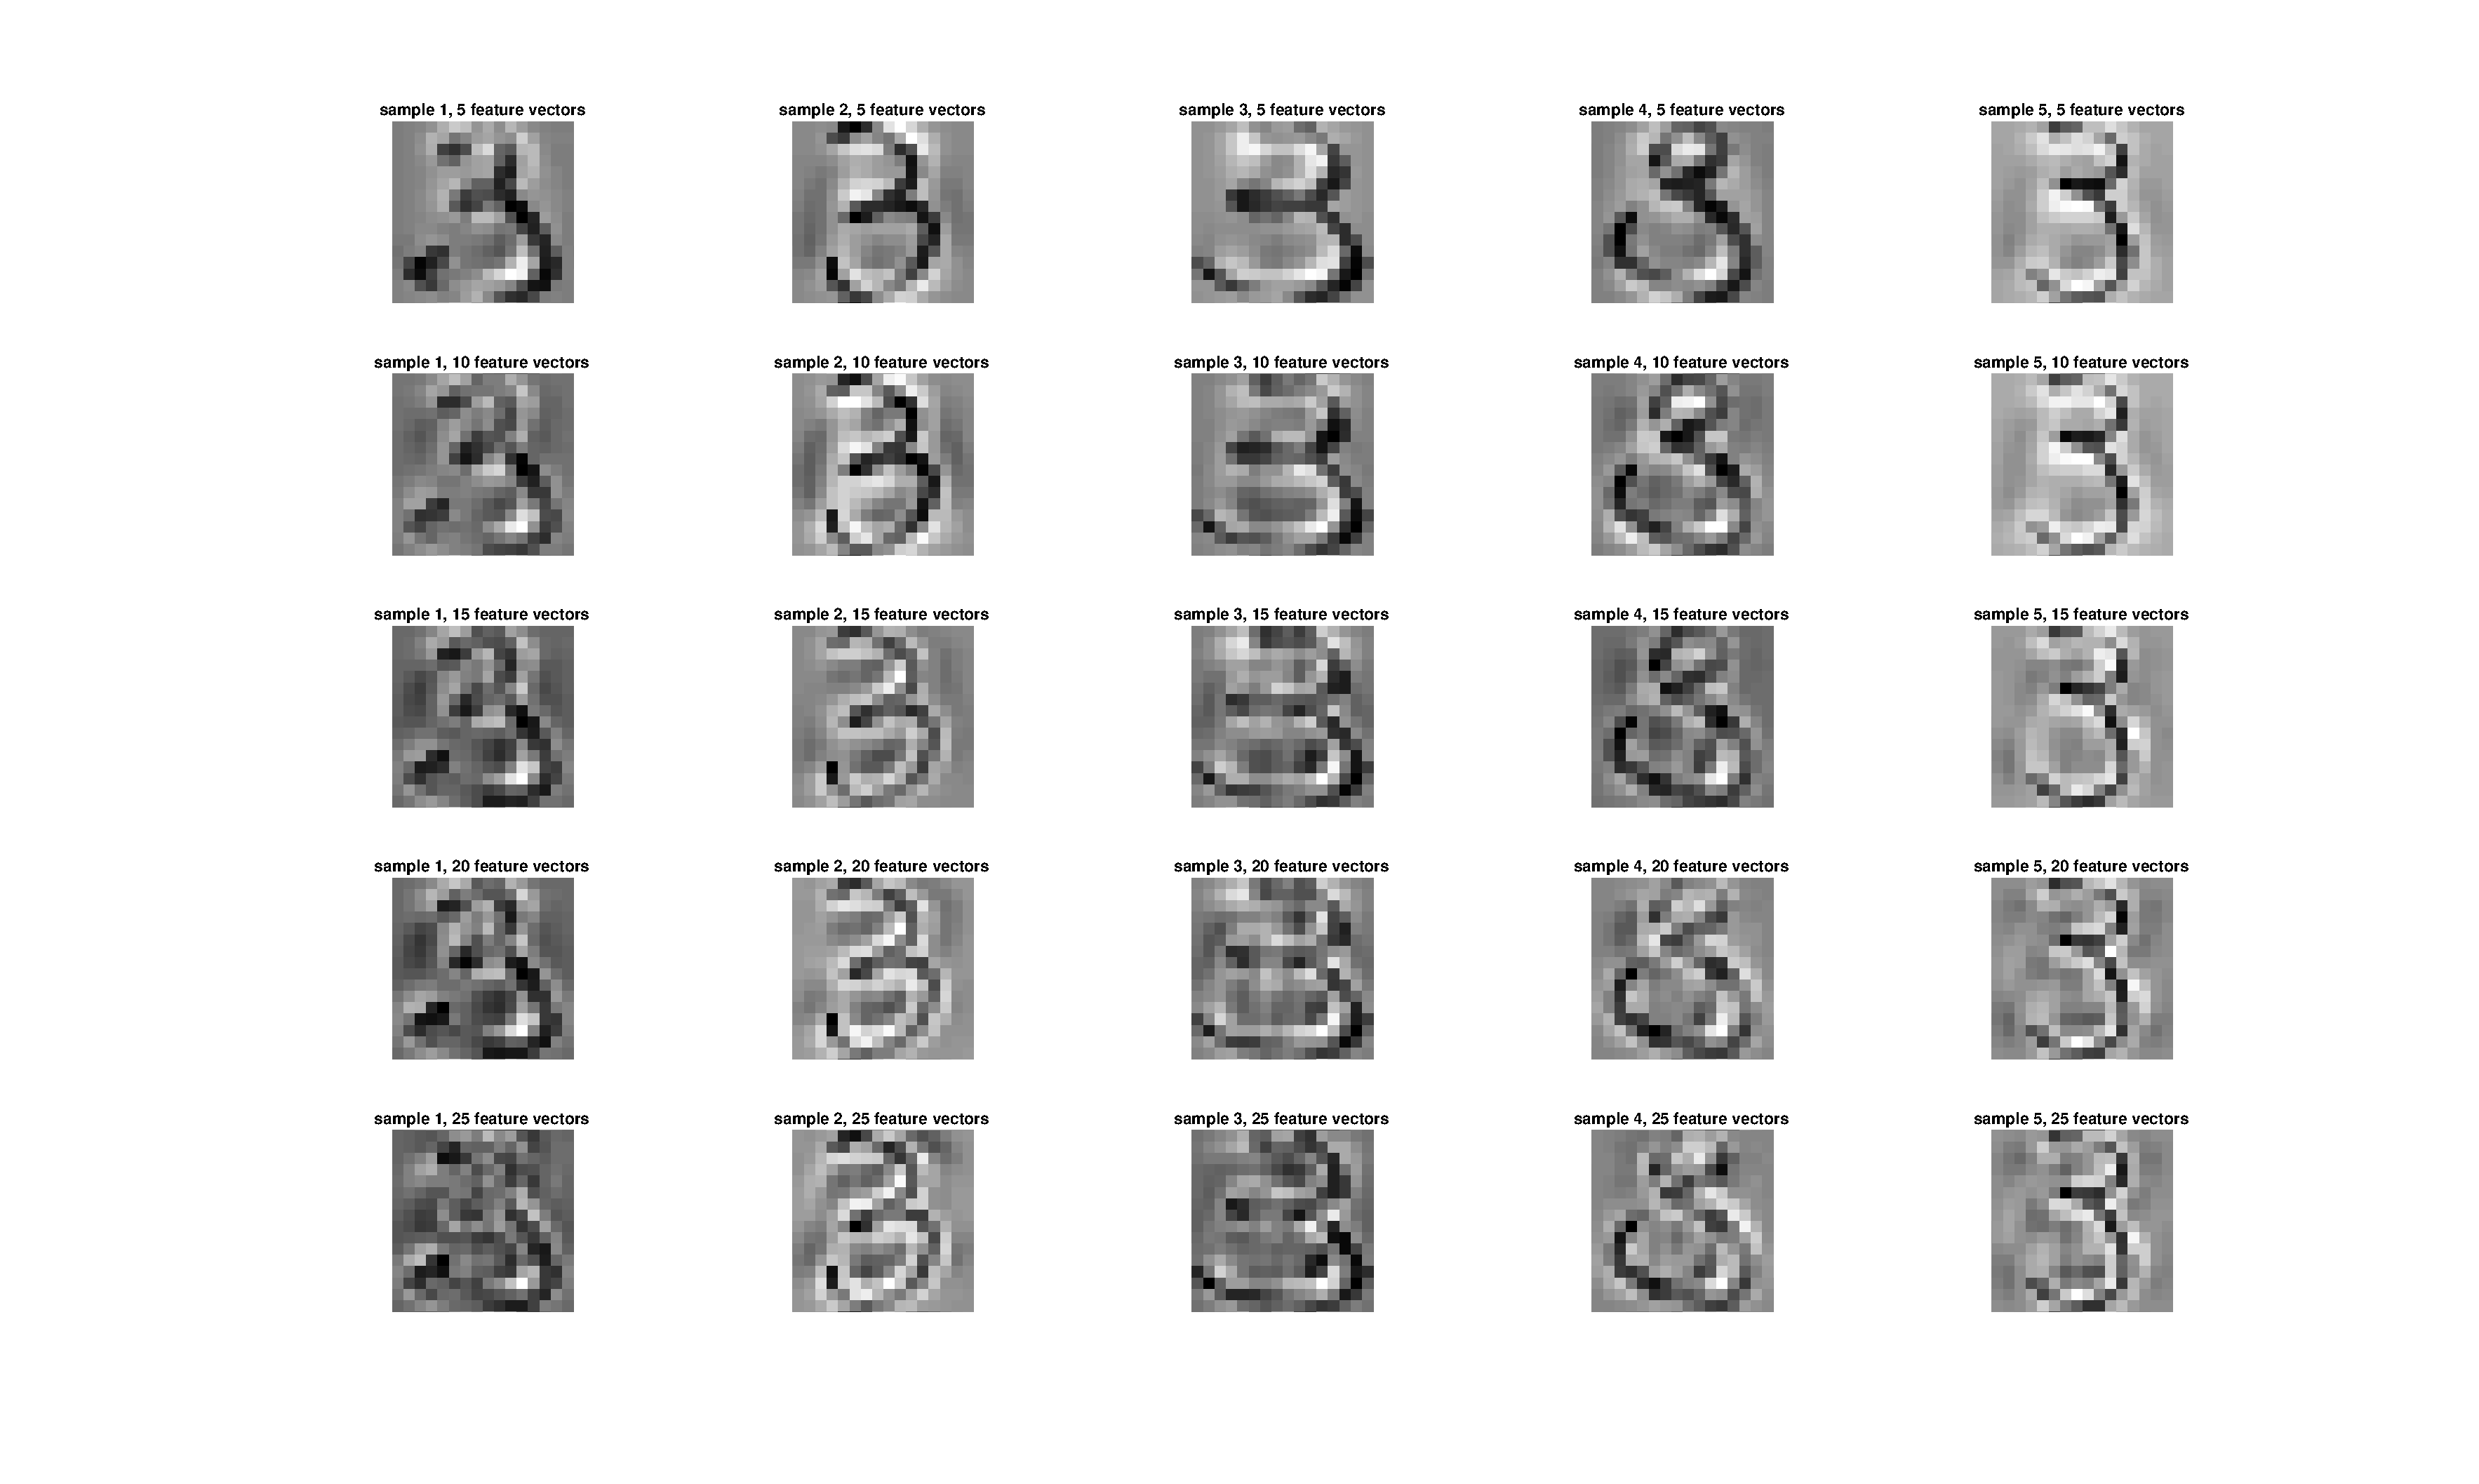
\includegraphics[width=10cm, height=8cm]{Q_2_3_residual}
        }
        \caption{\label{fig:my figure}  In the left panel the approximation of 5 samples of digit 3 using an increasing number of feature vectors.  Each column is a sample image, and the number of feature vectors increases from k=5:25 moving down the column.  The right panel shows the residuals in the same fashion.}
    \end{figure}
    
    \begin{figure}[!h]
        \centerline
        {
        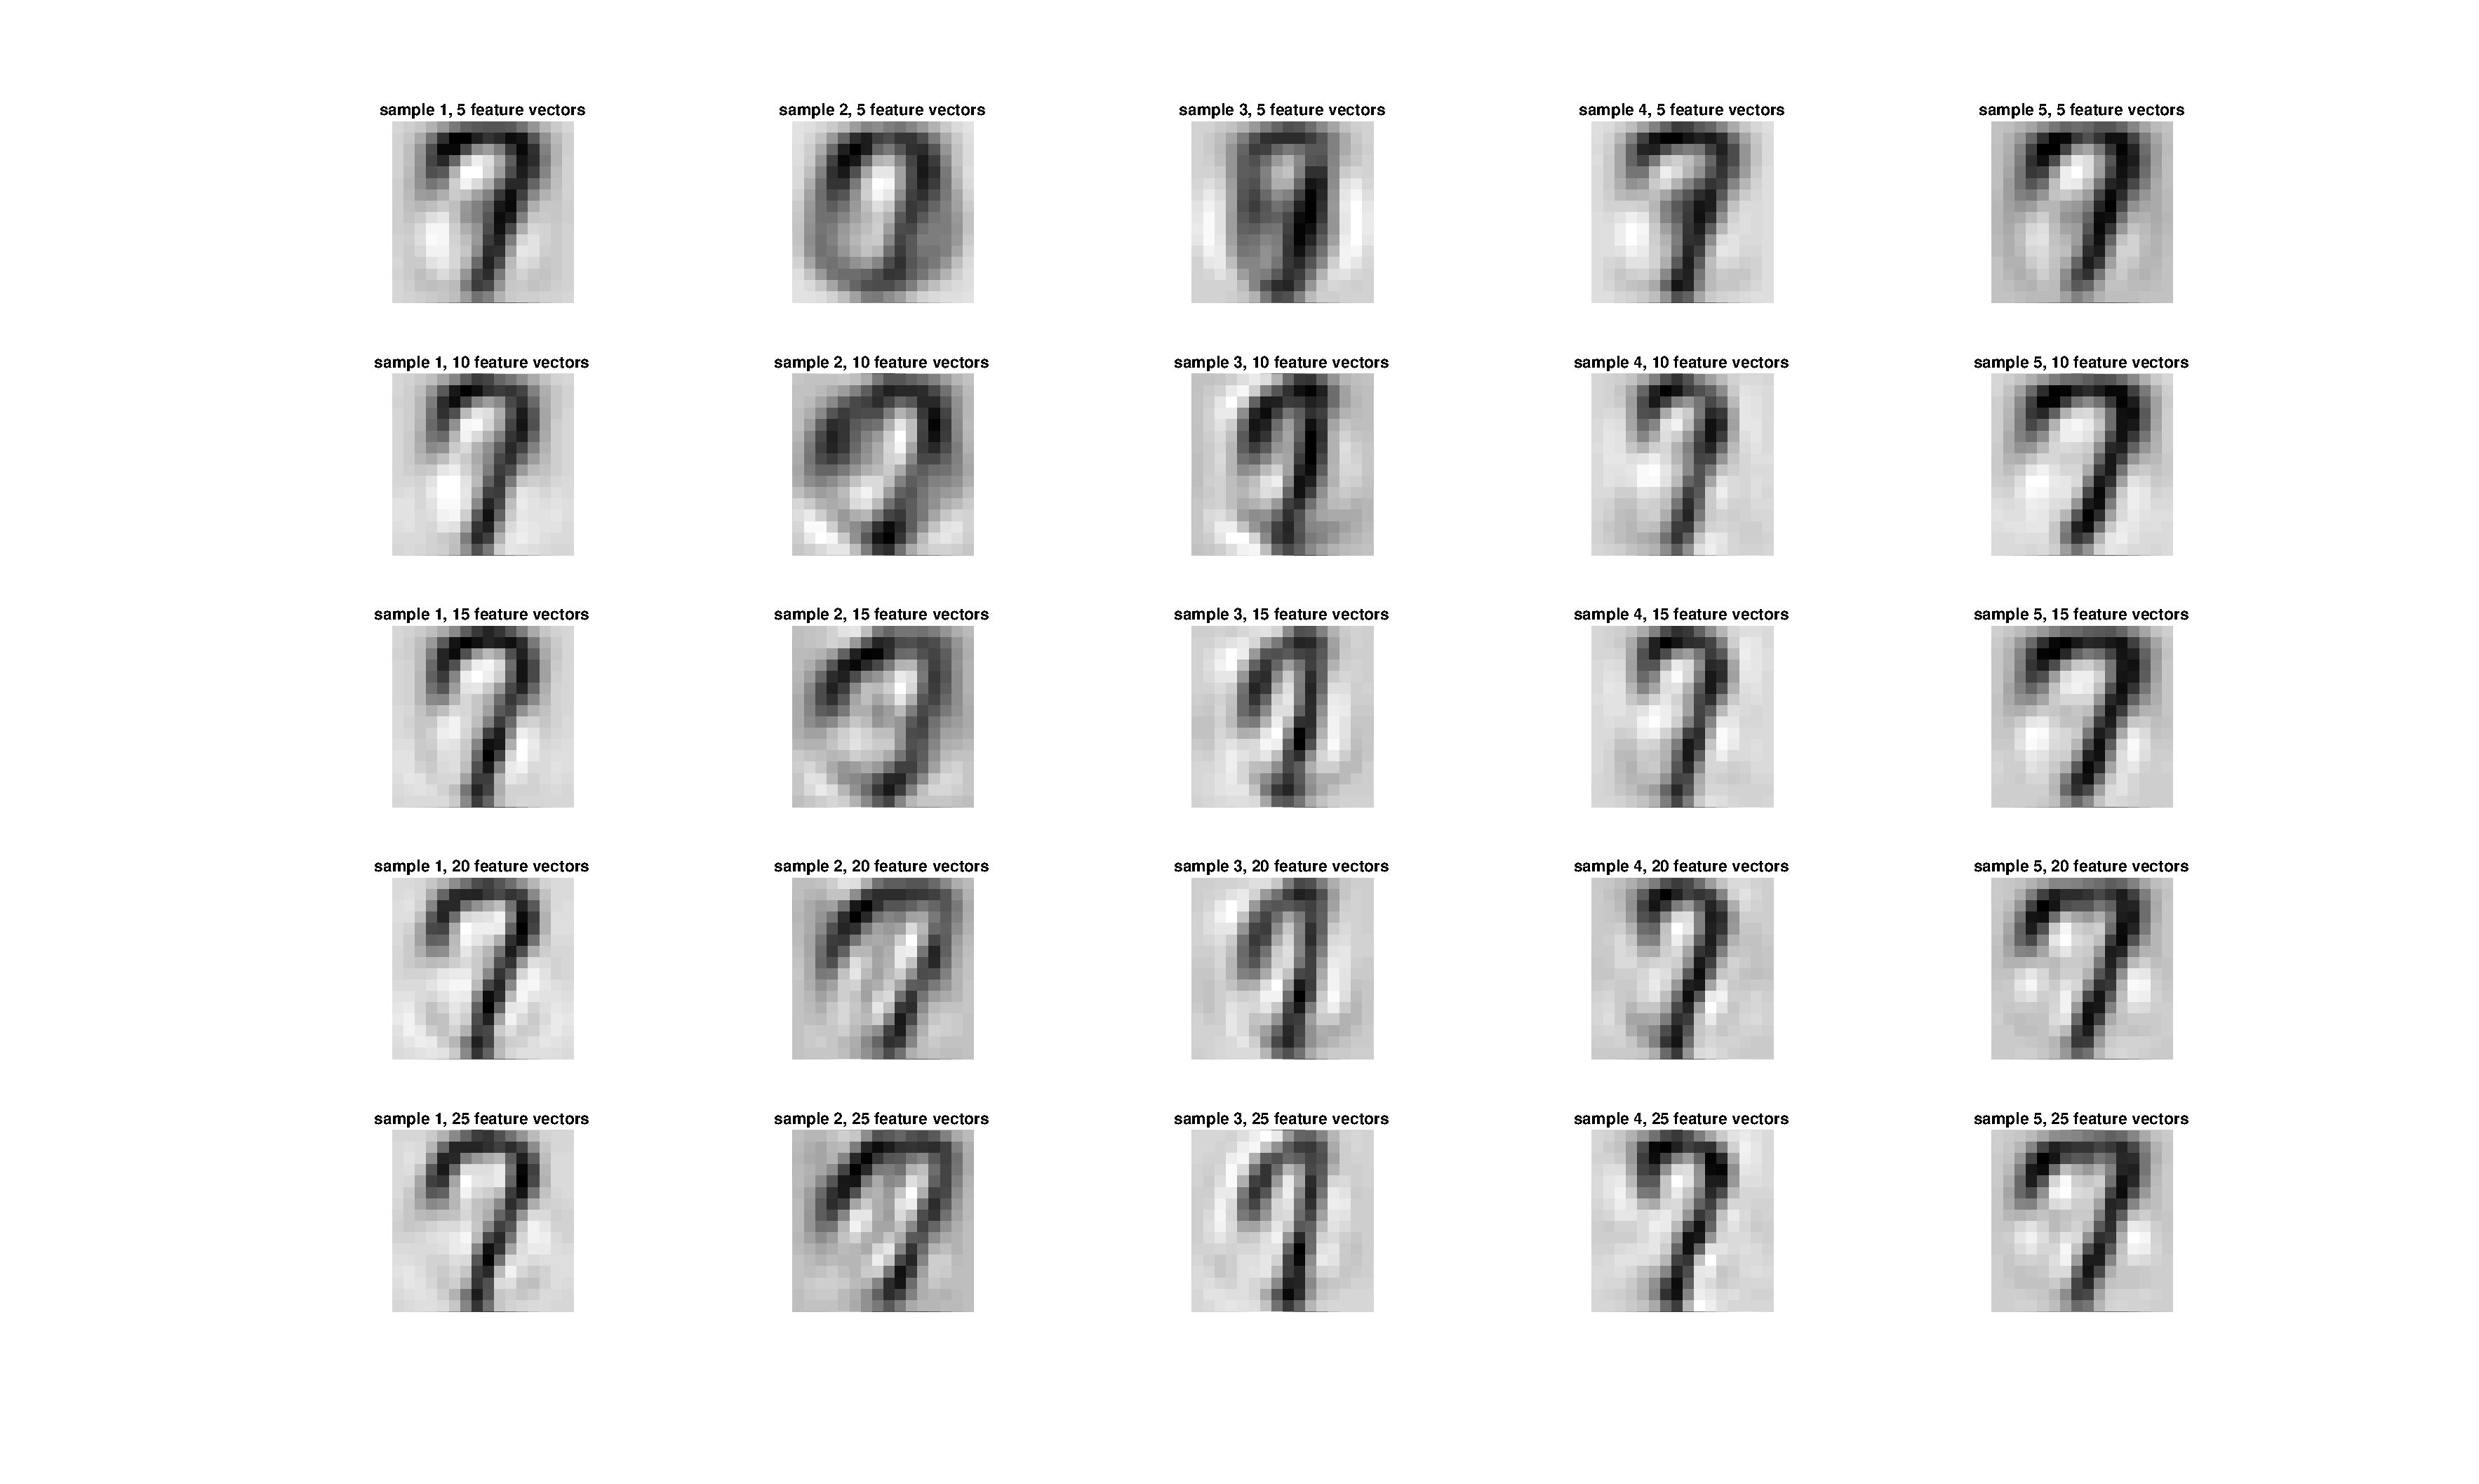
\includegraphics[width=10cm, height=8cm] {Q_2_7_approx}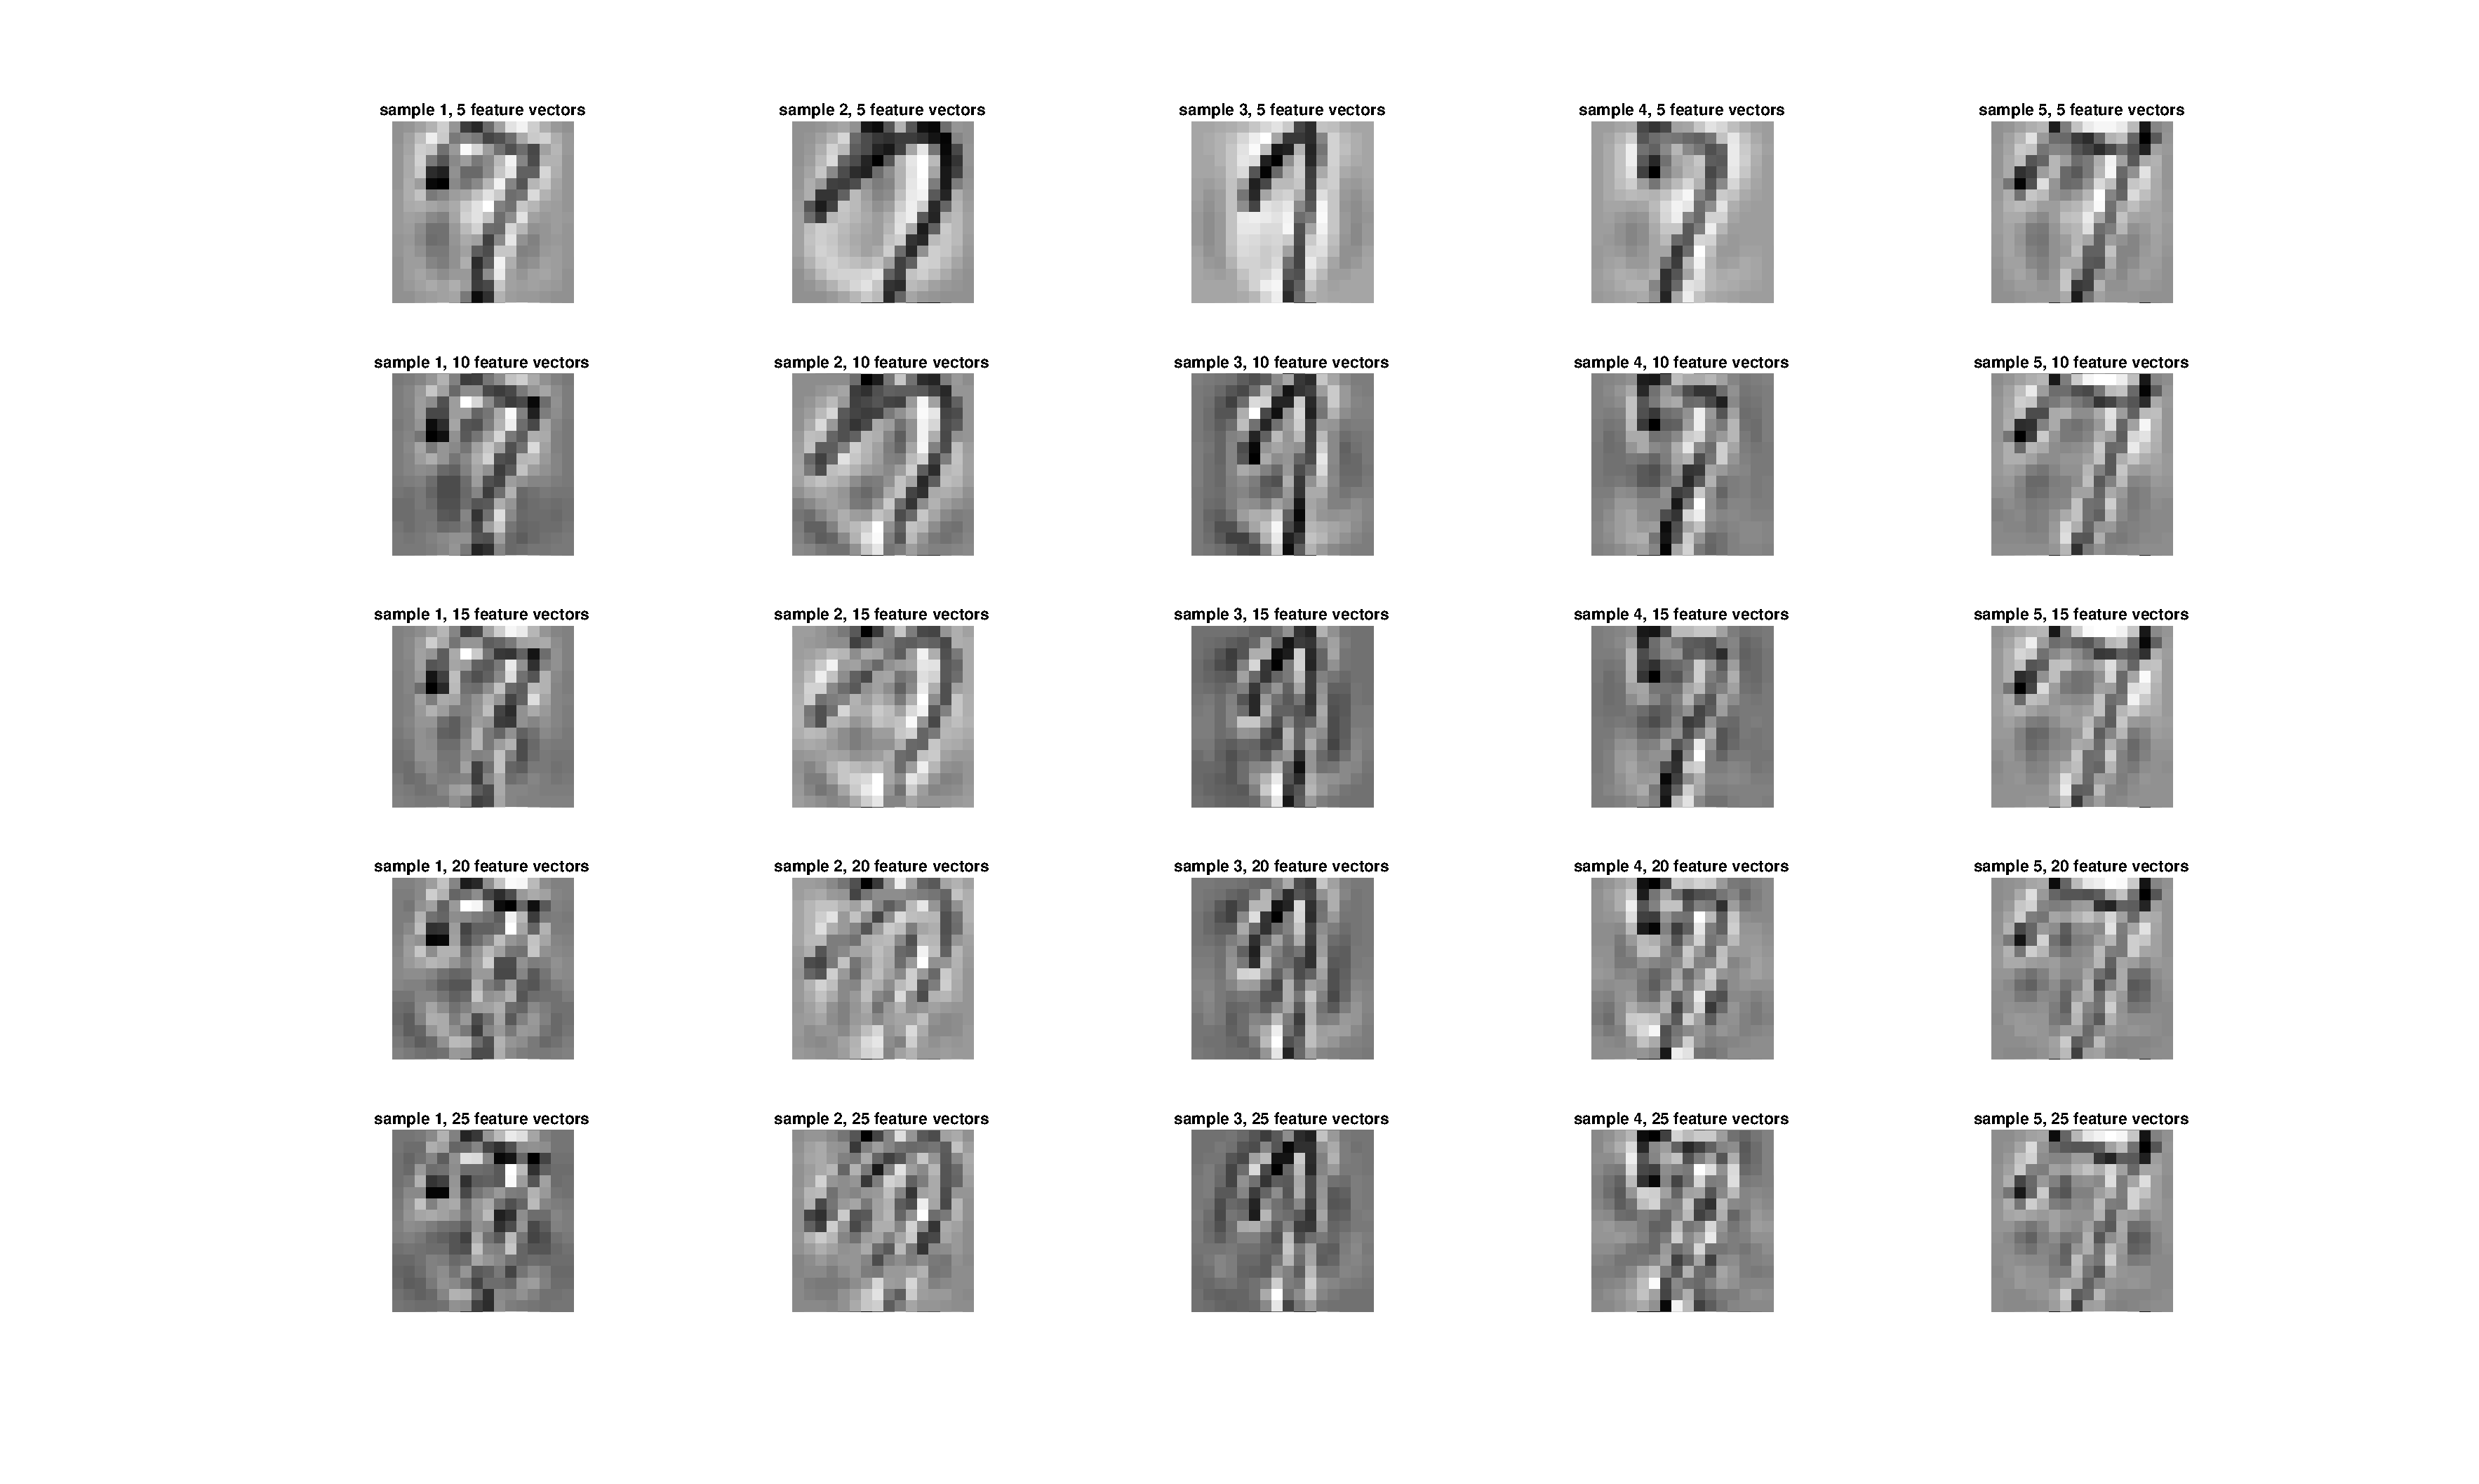
\includegraphics[width=10cm, height=8cm]{Q_2_7_residual}
        }
        \caption{\label{fig:my figure}  In the left panel the approximation of 5 samples of digit 7 using an increasing number of feature vectors.  Each column is a sample image, and the number of feature vectors increases from k=5:25 moving down the column.  The right panel shows the residuals in the same fashion. }
    \end{figure}

Figures 4, 5, 6, and 7 show in the left panel the approximation of 5 samples using an increasing number of feature vectors.  Each column is a sample image, and the number of feature vectors increases from k=5:25 moving down the column.  The right panel shows the residuals in the same fashion.  We can see that the first element of each column in the approximation plots look like generic forms of the number.  This is because it uses the smallest number of principal components, so approximates the number rougher and thereby gets at the heart of the number and loses the human hand of it.  As we move down columns the approximations get more human like and more accurate which makes sense.  The residual plots show the reverse effects which makes sense because the finer the approximation gets, the less fine its inverse with respect to the image should get.

\subsection*{Plot Norms of Errors}
Lastly, we calculate the error as a function of k.  To do so, I analyze the residual data because this represents what our approximation missed.  For each digit I calculate the 2-norm of the residuals over the 5 samples to yield a 1x5 vector storing the residual at k=5:25.  I plot the residual data as a function of k for each of the 4 digits in figure 8.  We can see that 1 has the least amount of error which makes sense because it is the easiest to approximate.  Followed by 7, 0, and 3 (which hold very similar values) which makes intuitive sense.  Also note that the error decreases inverse logarithmically with respect to increasing k which makes sense because as k increases from 0, each k value changes the approximation, and thereby the residual, a lot.  As k gets large, though, it has less bearing on the approximation/residual, which is why the graphs begin to flatten.  

    \begin{figure}[!h]
        \centerline
        {
        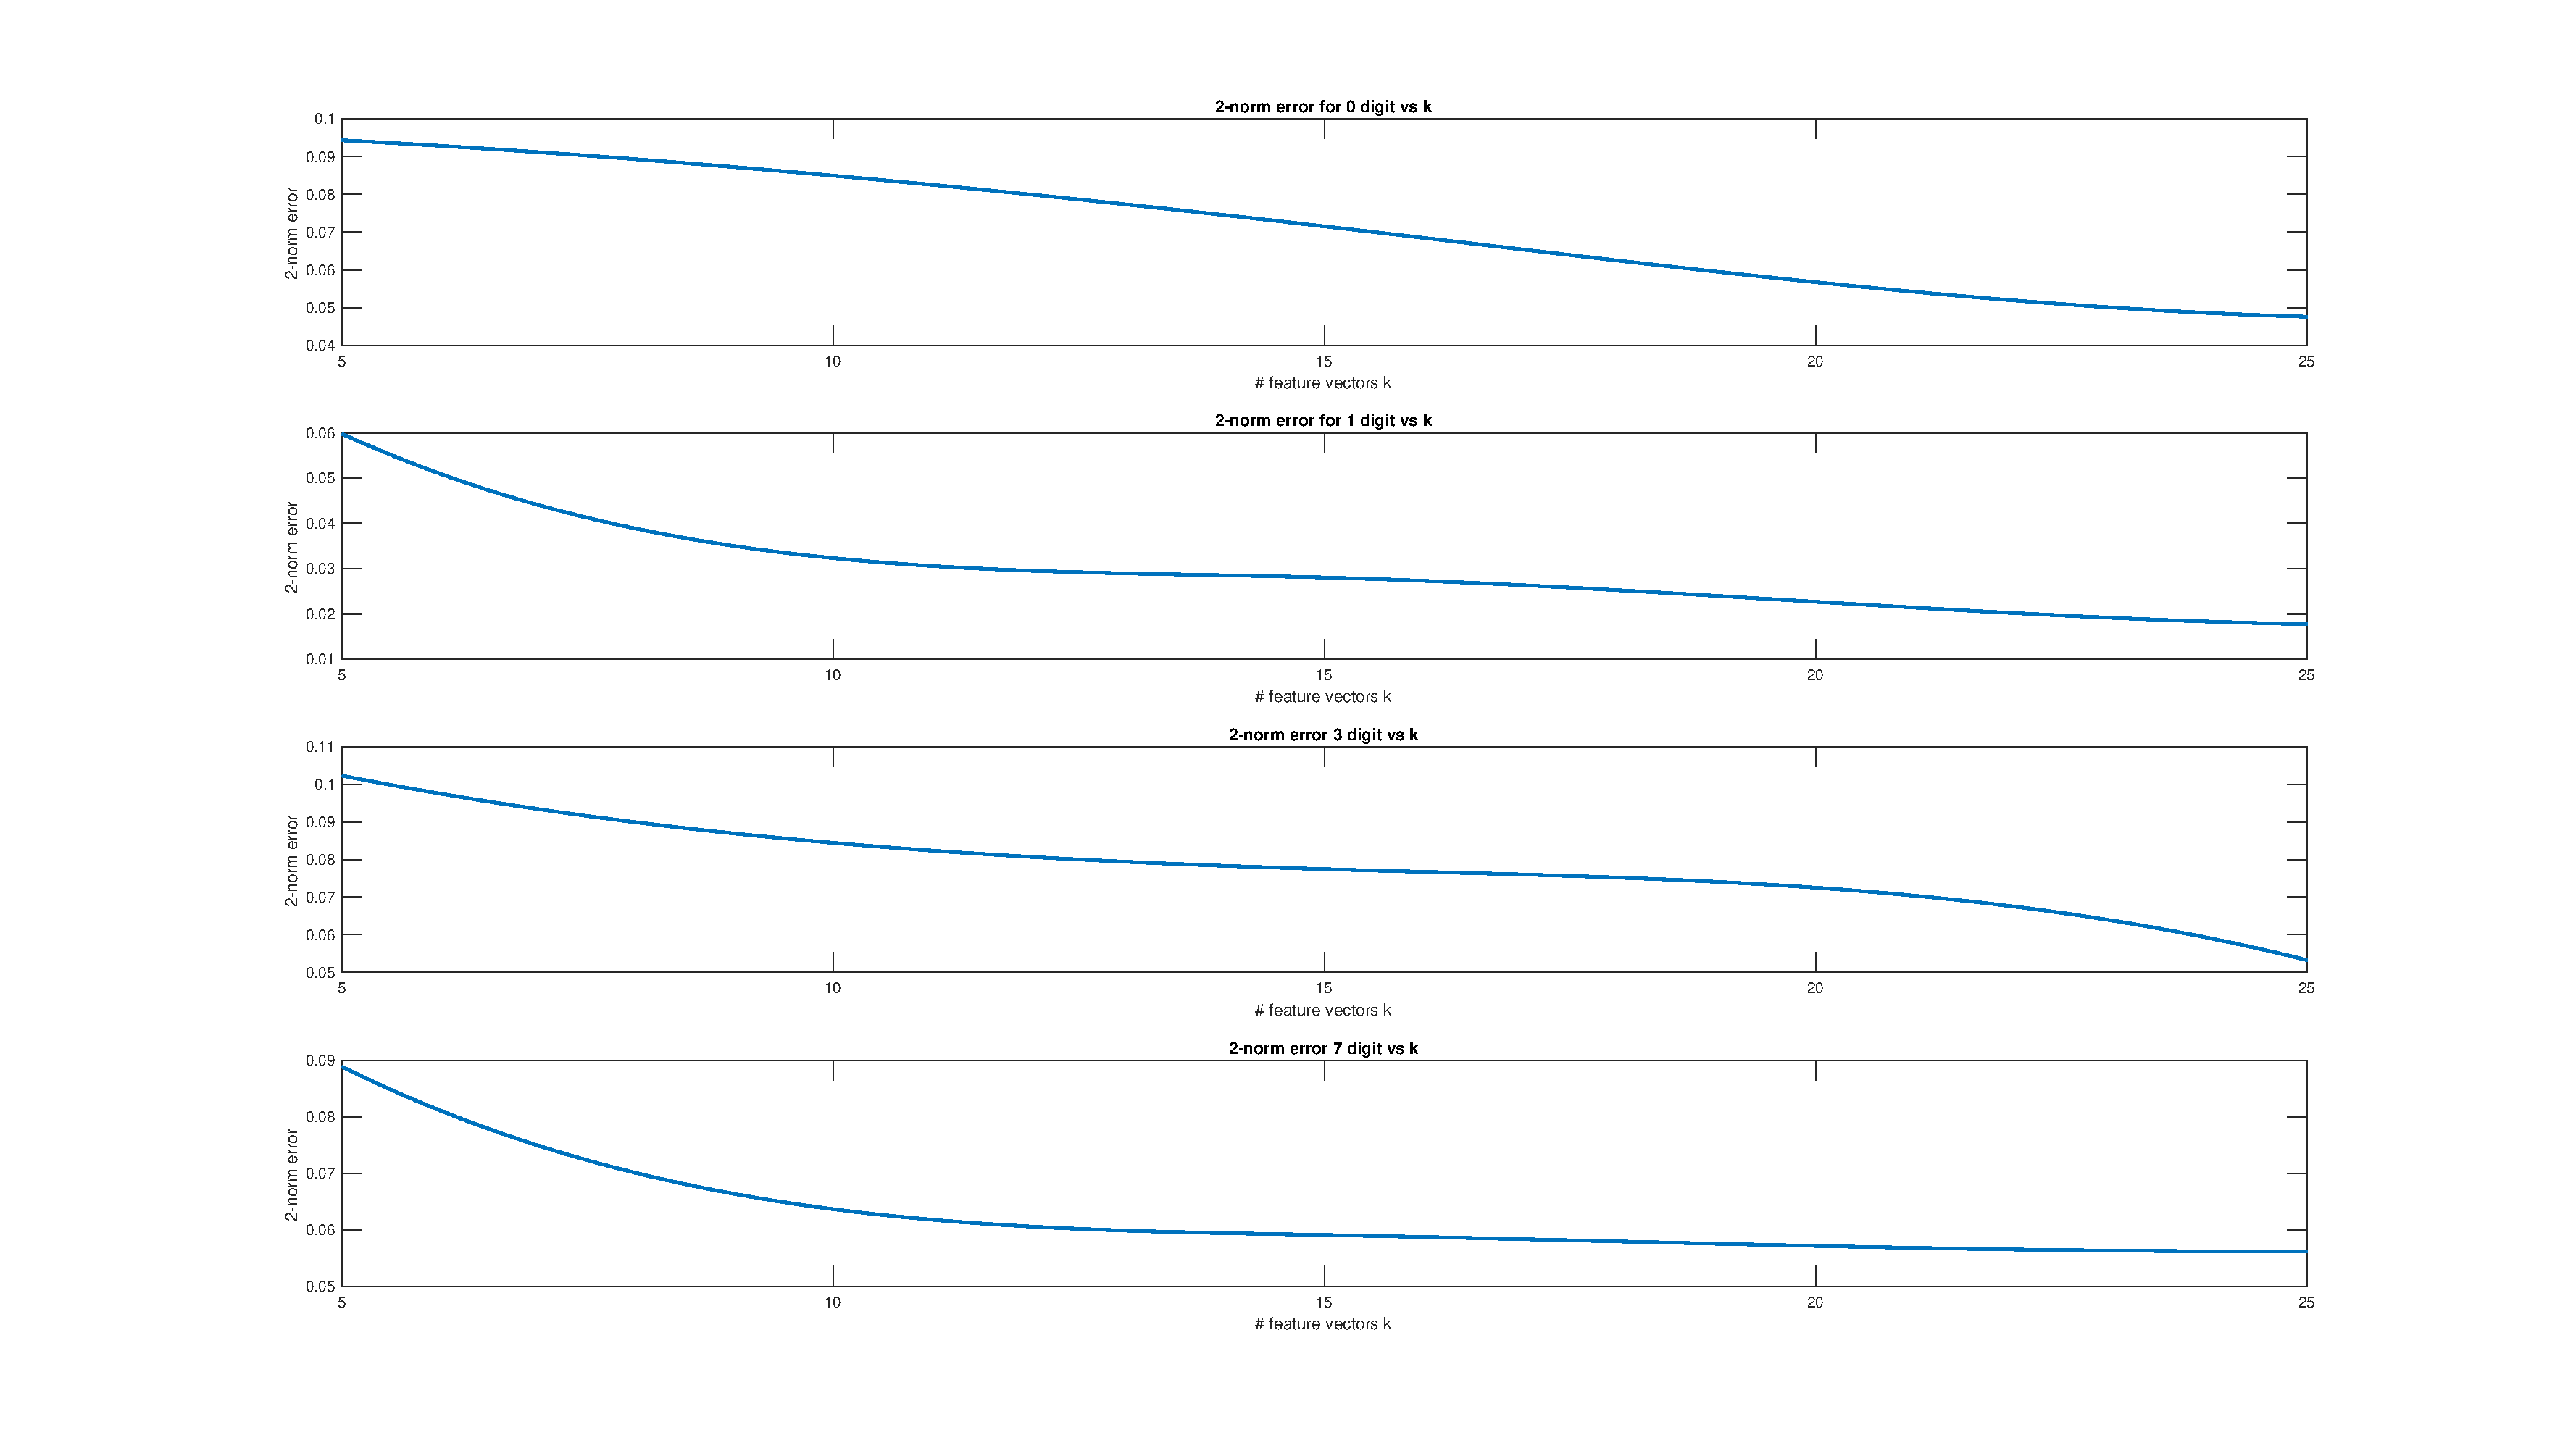
\includegraphics[width=15cm, height=12cm] {Q_2_error}
        }
        \caption{\label{fig:my figure}  2-norms of error as a function of # feature vectors k from 5:25 for digits 0, 1, 3, and 7}
    \end{figure}
    
\pagebreak
\section*{Problem 3}
\subsection*{Overview}
This problem asks us to analyze the iris data set from the 'IrisData.mat' file.  The iris data set is a matrix corresponding to flower characteristics for three types of flowers: iris setosa, iris versacolor, and iris virginica.  The algorithm relies on the data file 'IrisDataAnnotated.mat' which contains two matrices: Data matrix X which contains sepal length/width and petal length/width of 150 flowers.  And annotation vector I which indicates Iris species such that:
1= Iris setosa;     2=Iris versacolor;      3=Iris virginica\\
We will use PCA to determine if the data suggests the presence of clusters, similar to problem 1.  

\subsection*{PCA Analysis}
To begin, we center the data as in problem 1 by calculating the mean and subtracting the mean from each point.  Next we calculate the SVD. This returns a D matrix with diagonal values [95.95, 17.72, 3.47, 1.88].  This suggests that the data can be modeled well by 2 singular values.  I do plots including the 3rd for completeness in figure 9.  The graphs very clearly show the presence of two clusters. We know there are really 3 clusters, but the third is not so clear, that is what makes the data set so good for learning clustering!
    \begin{figure}[!h]
        \centerline
        {
        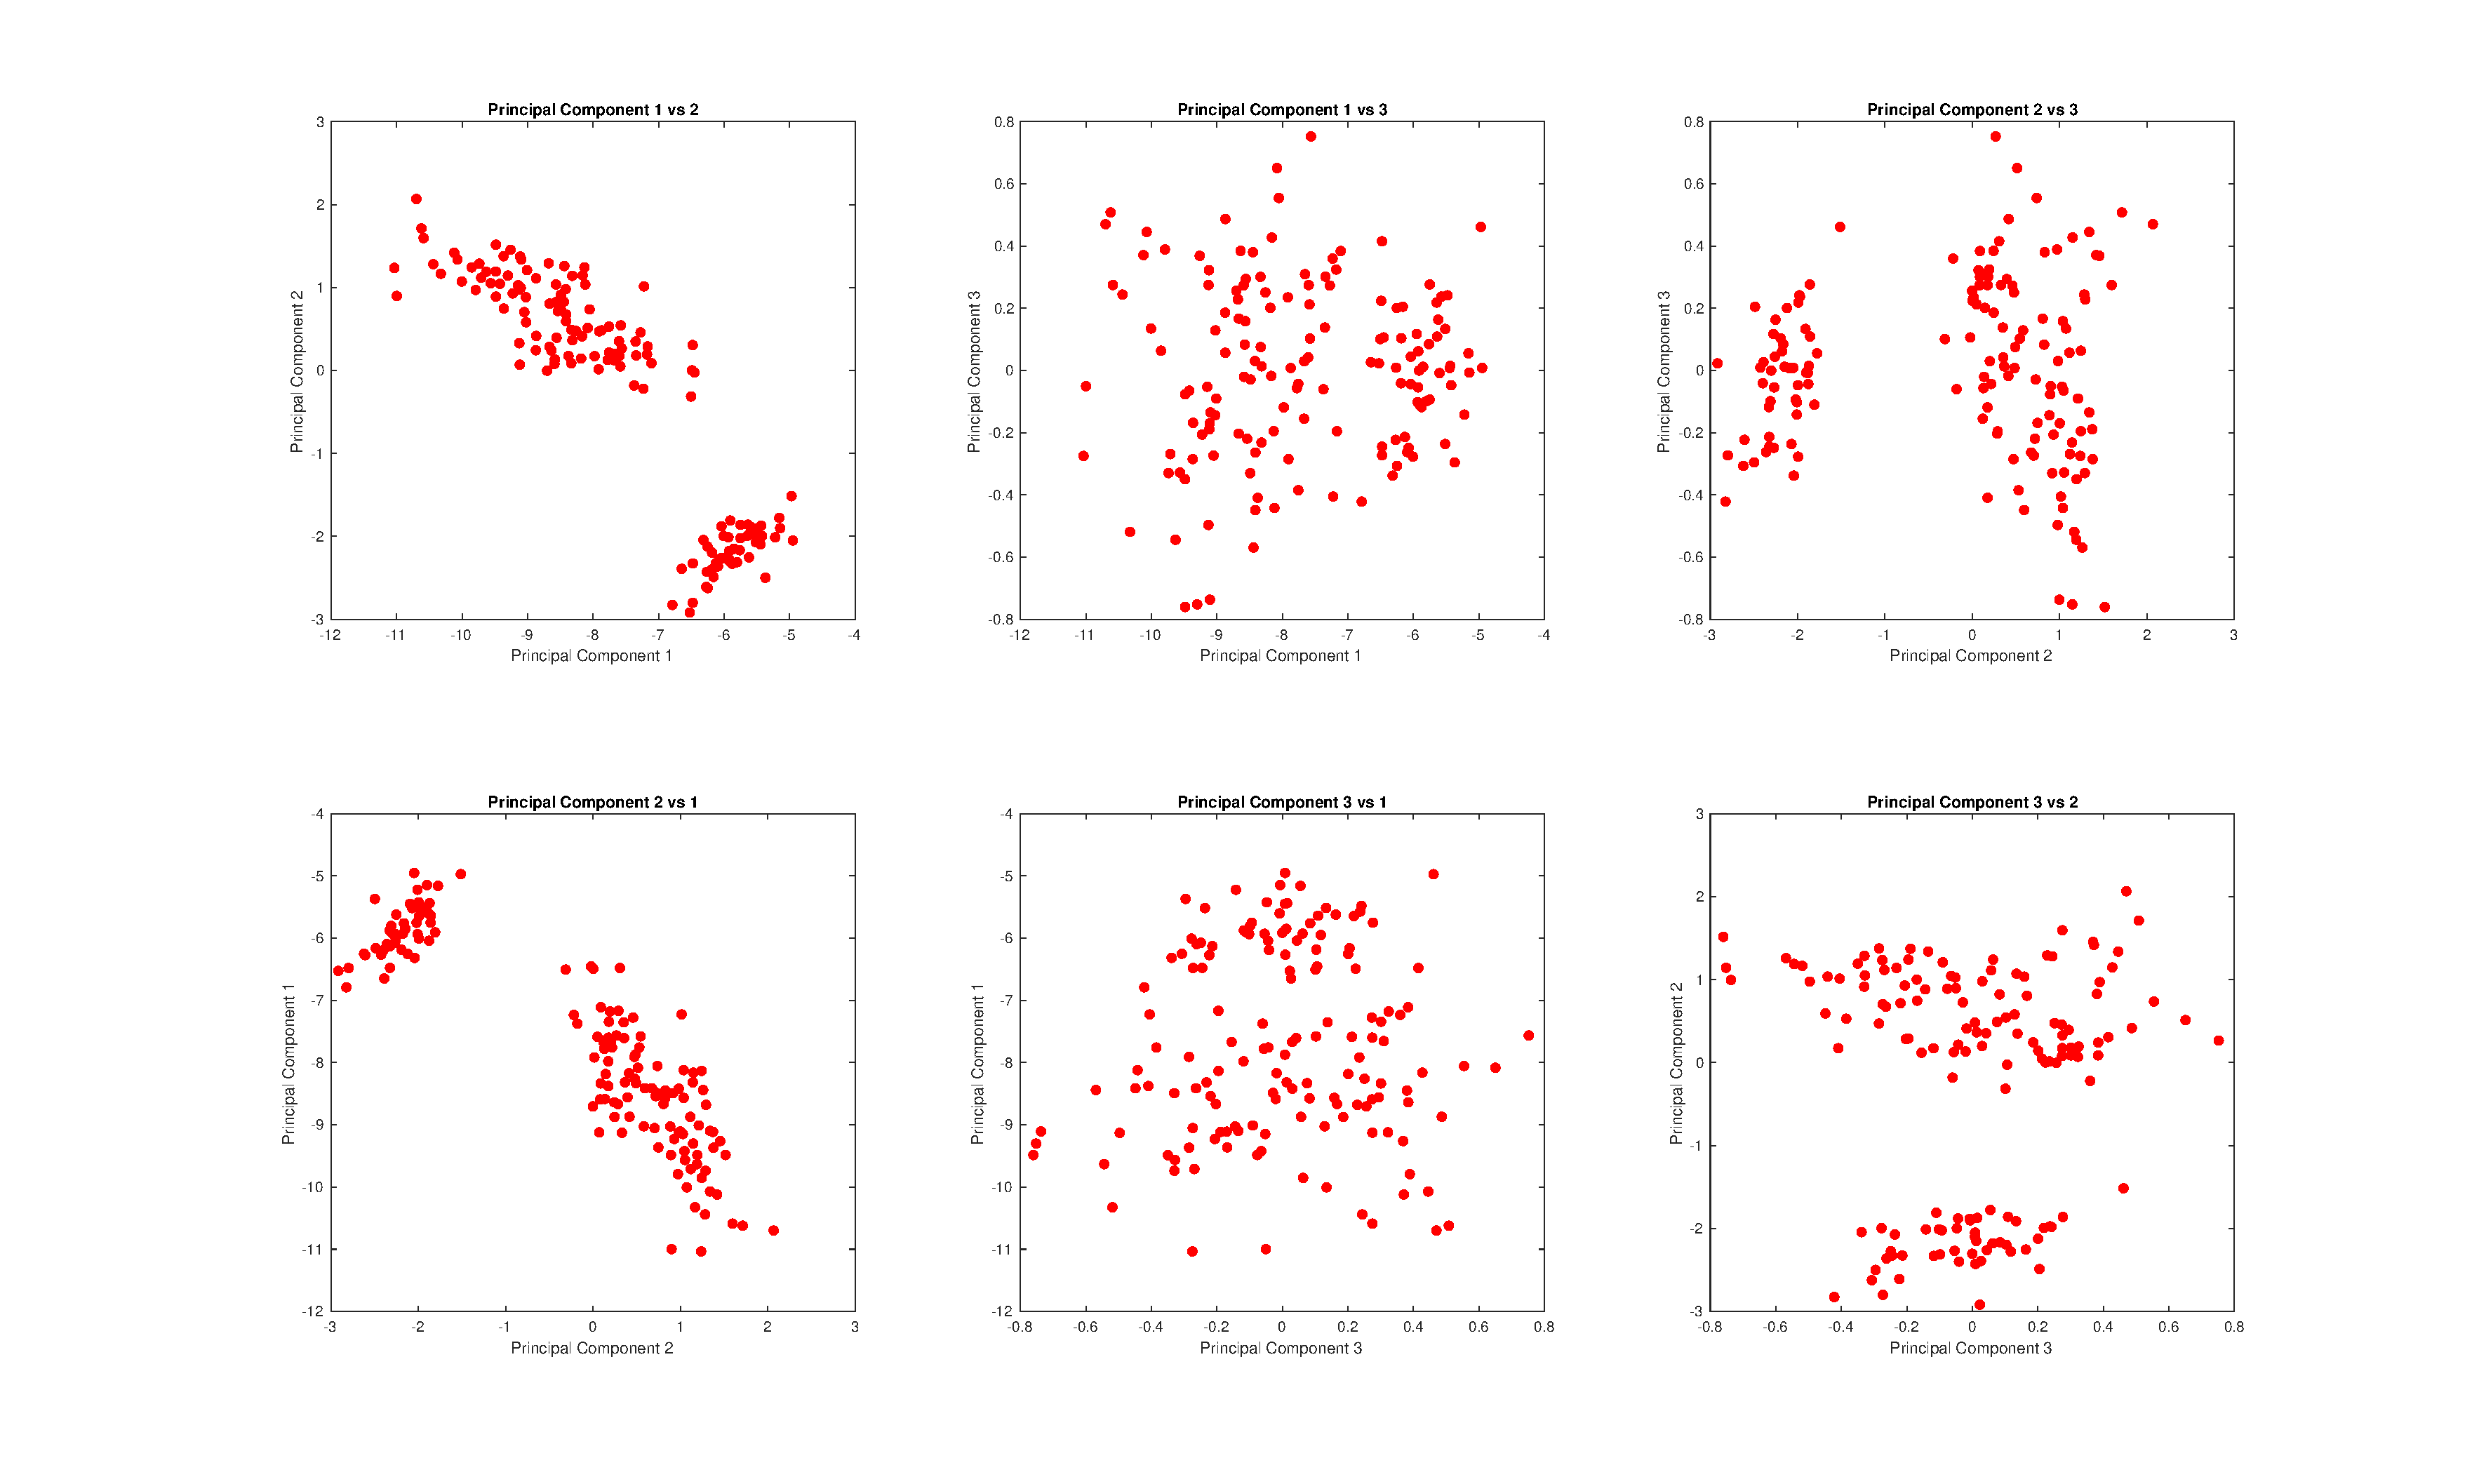
\includegraphics[width=15cm, height=11cm] {Q_3_3fv}
        }
        \caption{\label{fig:my figure} First three feature vectors plotted against each other. Clearly suggests existence of clusters}
    \end{figure}

\clearpage
\section*{Appendix 1: Problem 1 Matlab Code}
\begin{verbatim}
load ModelReductionData;
counter=1;
figure(1)
for i=1:5
    for j=i+1:6
        subplot(5,3,counter)
        plot(X(i,:),X(j,:), 'k.', 'MarkerSize',7);
        axis('equal');
        set(gca,'FontSize',20);
        counter=counter+1;
        title(['plot of dimension  ' num2str(i) ' vs dimension ' num2str(j)])
        xlabel(['dim ' num2str(i)]);
        ylabel(['dim ' num2str(j)]);
        
    end
end

[n,p]=size(X);
x_c = (1/p)*sum(X(:,:),2);
X_c = X - x_c*ones(1,p);

[U,D,V]=svd(X_c, 'econ');

d = diag(D);
figure(2);
semilogy(d,'k.','MarkerSize',20);
set(gca,'FontSize',20);
xlabel('Dimension Number');
ylabel('Singular Value');
title('Singular Values of X')

Z=U(:,1:3)'*X;


figure(3);
subplot(2,3,1)
plot(Z(1,1:4000),Z(2,1:4000),'r.','MarkerSize',20);
xlabel('Principal Component 1')
ylabel('Principal Component 2')
title('Principal Component 1 vs 2')

subplot(2,3,2)
plot(Z(1,1:4000),Z(3,1:4000),'r.','MarkerSize',20);
xlabel('Principal Component 1')
ylabel('Principal Component 3')
title('Principal Component 1 vs 3')

subplot(2,3,3)
plot(Z(2,1:4000),Z(3,1:4000),'r.','MarkerSize',20);
xlabel('Principal Component 2')
ylabel('Principal Component 3')
title('Principal Component 2 vs 3')

subplot(2,3,4)
plot(Z(2,1:4000),Z(1,1:4000),'r.','MarkerSize',20);
xlabel('Principal Component 2')
ylabel('Principal Component 1')
title('Principal Component 2 vs 1')

subplot(2,3,5)
plot(Z(3,1:4000),Z(1,1:4000),'r.','MarkerSize',20);
xlabel('Principal Component 3')
ylabel('Principal Component 1')
title('Principal Component 3 vs 1')

subplot(2,3,6)
plot(Z(3,1:4000),Z(2,1:4000),'r.','MarkerSize',20);
xlabel('Principal Component 3')
ylabel('Principal Component 2')
title('Principal Component 3 vs 2')
\end{verbatim}

\pagebreak
\section*{Appendix 2: Problem 2 Matlab Code}
\begin{verbatim}
load HandwrittenDigits X I;

X_0=X(:,(find(I==0)));
[U,S,V]=svd(X,'econ');
residual_x_0=zeros(256,5);
for i=1:5
    for k=1:5
        z=U(:,1:5*k)'*X_0(:,i);
        reconstructed_x_0= U(:,1:5*k)*z;
        this_residual_0 = X_0(:,i)-reconstructed_x_0;
        residual_x_0(:,k)=residual_x_0(:,k) + this_residual_0;

        figure(1);
        subplot(5,5,5*(k-1)+i);
        imagesc(reshape(reconstructed_x_0,16,16)');
        colormap(1-gray);
        axis('square');
        axis('off');
        title(['sample ' num2str(i) ', ' num2str(5*k) ' feature vectors'])
        
        figure(2);
        subplot(5,5,5*(k-1)+i);
        imagesc(reshape(this_residual_0,16,16)');
        colormap(1-gray);
        axis('square');
        axis('off');  
        title(['sample ' num2str(i) ', ' num2str(5*k) ' feature vectors'])

    end
end
residual_x_0=sum(sqrt(((residual_x_0/5).^2)))*(1/256);


X_1=X(:,(find(I==1)));
[U,S,V]=svd(X,'econ');
residual_x_1=zeros(256,5);
for i=1:5
    for k=1:5
        z=U(:,1:5*k)'*X_1(:,i);
        reconstructed_x_1= U(:,1:5*k)*z;
        this_residual_1 = X_1(:,i)-reconstructed_x_1;
        residual_x_1(:,k)=residual_x_1(:,k) + this_residual_1;

        figure(3);
        subplot(5,5,5*(k-1)+i);
        imagesc(reshape(reconstructed_x_1,16,16)');
        colormap(1-gray);
        axis('square');
        axis('off');
        title(['sample ' num2str(i) ', ' num2str(5*k) ' feature vectors'])
        
        
        figure(4);
        subplot(5,5,5*(k-1)+i);
        imagesc(reshape(this_residual_1,16,16)');
        colormap(1-gray);
        axis('square');
        axis('off');   
        title(['sample ' num2str(i) ', ' num2str(5*k) ' feature vectors'])
    end
end
residual_x_1=sum(sqrt(((residual_x_1/5).^2)))*(1/256);


X_3=X(:,(find(I==3)));
[U,S,V]=svd(X,'econ');
residual_x_3=zeros(256,5);
for i=1:5
    for k=1:5
        z=U(:,1:5*k)'*X_3(:,i);
        reconstructed_x_3= U(:,1:5*k)*z;
        this_residual_3 = X_3(:,i)-reconstructed_x_3;
        residual_x_3(:,k)=residual_x_3(:,k) + this_residual_3;

        figure(5);
        subplot(5,5,5*(k-1)+i);
        imagesc(reshape(reconstructed_x_3,16,16)');
        colormap(1-gray);
        axis('square');
        axis('off');
        title(['sample ' num2str(i) ', ' num2str(5*k) ' feature vectors'])
        
        figure(6);
        subplot(5,5,5*(k-1)+i);
        imagesc(reshape(this_residual_3,16,16)');
        colormap(1-gray);
        axis('square');
        axis('off'); 
        title(['sample ' num2str(i) ', ' num2str(5*k) ' feature vectors'])
    end
end
residual_x_3=sum(sqrt(((residual_x_3/5).^2)))*(1/256);


X_7=X(:,(find(I==7)));
[U,S,V]=svd(X,'econ');
residual_x_7=zeros(256,5);
for i=1:5
    for k=1:5
        z=U(:,1:5*k)'*X_7(:,i);
        reconstructed_x_7= U(:,1:5*k)*z;
        this_residual_7 = X_7(:,i)-reconstructed_x_7;
        residual_x_7(:,k)=residual_x_7(:,k) + this_residual_7;

        figure(7);
        subplot(5,5,5*(k-1)+i);
        imagesc(reshape(reconstructed_x_7,16,16)');
        colormap(1-gray);
        axis('square');
        axis('off');
        title(['sample ' num2str(i) ', ' num2str(5*k) ' feature vectors'])
            
        figure(8);
        subplot(5,5,5*(k-1)+i);
        imagesc(reshape(this_residual_7,16,16)');
        colormap(1-gray);
        axis('square');
        axis('off'); 
        title(['sample ' num2str(i) ', ' num2str(5*k) ' feature vectors'])
    end
end
residual_x_7=sum(sqrt(((residual_x_7/5).^2)))*(1/256);


residuals=[residual_x_0; residual_x_1; residual_x_3; residual_x_7];
k=[5 10 15 20 25];
for z=1:4
    figure(9);
    subplot(4,1,z);
    scatter(k,residuals(z,:), 'linewidth', 1.5);
    fnplt(csapi(k,residuals(z,:)))
end

figure(9);
subplot(4,1,1);
title('2-norm error for 0 digit vs k');
xlabel('# feature vectors k')
ylabel('2-norm error')
subplot(4,1,2);
title('2-norm error for 1 digit vs k');
xlabel('# feature vectors k')
ylabel('2-norm error')
subplot(4,1,3);
title('2-norm error 3 digit vs k');
xlabel('# feature vectors k')
ylabel('2-norm error')
subplot(4,1,4);
title('2-norm error 7 digit vs k');
xlabel('# feature vectors k')
ylabel('2-norm error')


\end{verbatim}

\pagebreak
\section*{Appendix 3: Problem 3 Matlab Code}
\begin{verbatim}
load IrisData;

[n,p]=size(X);
x_c = (1/p)*sum(X(:,:),2);
X_c = X - x_c*ones(1,p);
[U,D,V]=svd(X,'econ');
Z=U(:,1:3)'*X;

figure(1);
subplot(2,3,1)
plot(Z(1,:),Z(2,:),'r.','MarkerSize',20);
xlabel('Principal Component 1')
ylabel('Principal Component 2')
title('Principal Component 1 vs 2')

subplot(2,3,2)
plot(Z(1,:),Z(3,:),'r.','MarkerSize',20);
xlabel('Principal Component 1')
ylabel('Principal Component 3')
title('Principal Component 1 vs 3')

subplot(2,3,3)
plot(Z(2,:),Z(3,:),'r.','MarkerSize',20);
xlabel('Principal Component 2')
ylabel('Principal Component 3')
title('Principal Component 2 vs 3')

subplot(2,3,4)
plot(Z(2,:),Z(1,:),'r.','MarkerSize',20);
xlabel('Principal Component 2')
ylabel('Principal Component 1')
title('Principal Component 2 vs 1')

subplot(2,3,5)
plot(Z(3,:),Z(1,:),'r.','MarkerSize',20);
xlabel('Principal Component 3')
ylabel('Principal Component 1')
title('Principal Component 3 vs 1')

subplot(2,3,6)
plot(Z(3,:),Z(2,:),'r.','MarkerSize',20);
xlabel('Principal Component 3')
ylabel('Principal Component 2')
title('Principal Component 3 vs 2')
\end{verbatim}

\end{document}


